\documentclass[12pt,oneside]{CUNY_PhD}

\pagestyle{headings}
\title{Finite Gaussian Neurons - A Defense Against Adversarial Attacks?}
\author{Felix Grezes}

% \usepackage{fullpage}
\usepackage{graphicx}
\usepackage{amssymb}
\usepackage{url}
\usepackage{epstopdf}
\usepackage{enumitem}
\usepackage{amsmath}
\usepackage{subcaption}


%% ...
%% any 'preamble' stuff
%% ...

\begin{document}

\frontmatter

\maketitle % same name as the 'book' documentclass command, but gives a CUNY titlepage

%% optional:
\makecopyrightpage

\makeapprovalpage{Pr.\ Michael I.\ Mandel}{Pr.\ Rivka Levitan}{Pr.\ Ioannis Stamos}{Dr.\ Andrew Rosenberg}

%% optional:
\makeabstractpage{Pr. Michael I. Mandel}{
Since 2014, artificial neural networks have been known to be vulnerable to adversarial attacks, which can imperceptibly alter inputs to fool the network into producing wrong or nonsensical outputs.

While defenses against adversarial attacks have been proposed, they usually involve retraining a new neural network from scratch, a costly task.

In this work, I introduce the Finite Gaussian Neuron\protect\footnote{The code used for this work is available at \url{https://github.com/grezesf/FGN---Research} under the GPL 3.0 open source licence. Work done with PyTorch.}, a novel neuron architecture for artificial neural networks.

My works aims to:
\begin{itemize}[itemsep=-4mm]
    \item easily convert existing models to Finite Gaussian Neuron architecture,
    \item while preserving the existing model's behavior on real data,
    \item and offering resistance against adversarial attacks.
\end{itemize}

\newpage % add space between this and footnote

I show that converted and retrained Finite Gaussian neural networks always have lower confidence in their predictions over randomized and FGSM adversarial images when compared to classical neural networks, while maintaining high accuracy and confidence over real MNIST images.

To further validate the capacity of Finite Gaussian Neurons to protect from adversarial attacks, I propose:
\begin{itemize}[itemsep=-4mm]
    \item evaluating the models on CIFAR-10 and SPEECHCOMMANDS,
    \item testing against the PGD and Carlini-Wagner adversarial attacks,
    \item testing against transferable and universal adversarial perturbations,
    \item and implementing an FGN version of the convolutional layer.
\end{itemize}
}
%% (In addition to these last four custom CUNY commands, all LaTex
%% commands, including those from the LaTeX 'book' class, are available.
%% Footnotes and the bibliography will be single spaced, as
%% required by CUNY, while the main text will be double spaced.)

%% optional:
% \chapter*{Acknowledgements}
%% Text of acknowledgements

\tableofcontents

\mainmatter

\chapter{Introduction}
% definitions? (will be introduced as needed)
% brief history? nn->attacks exist (what are attacks)
Artificial neurons, since their creation as the perceptron in 1958 by Frank Rosenblatt\cite{rosenblatt1958perceptron} and their practical integration into artificial neural  networks in 1975 by Paul Werbos\cite{werbos1975beyond}, are a fundamental building block of modern machine learning and artificial intelligence systems. Despite their success, artificial neural networks were shown in 2014 by Goodfellow et al.\cite{goodfellow2015explaining} to be vulnerable to adversarial attacks . These adversarial attack methods exploit unintuitive or misunderstood properties of artificial neural networks to generates adversarial examples, i.e., carefully crafted inputs that are capable of fooling these networks. These adversarial examples are often indistinguishable from normal inputs to humans. 
% For example, an adversarial attack might modify image of a cat, correctly recognized as such by the artificial neural network, into an image that the network erroneously recognizes as a dog with high confidence. 
Defenses against adversarial attacks have been proposed (survey in 2018 by Akhtar et al.\cite{akhtar2018threat}), but are either computationally expensive as in the case of adversarial re-training (Madry et al. 2019 \cite{madry2019deep}), or do not generalize well to novel attacks as in the case of network distillation (Papernot et al. 2016 \cite{Papernot2016DistillationAA}, Carlini et al. 2017  \cite{carlini2017evaluating}).

In this work I introduce the Finite Gaussian Neuron (FGN), a novel architecture for the artificial neuron. I show that artificial neural networks that incorporate the FGN architecture are resistant to adversarial attacks, while exhibiting another desirable property: they are naturally resistant to rubbish class inputs. Furthermore existing networks can be converted to the FGN architecture without any expensive computation while preserving the network's behavior over data.



\section{Motivation}
There are two main intuitions that motivate the Finite Gaussian Neuron, both of which might explain why neural networks are susceptible to adversarial attacks: the \emph{piece-wise linearity} of the artificial neurons and the \emph{curse of dimensionality}.

Typically, artificial neural networks are built by combining artificial neurons into layers, and these neurons individually separate their input space into linear contours, see Goodfellow et al. 2016 \cite{goodfellow2016deep}. The combination of these linear contours through stacked layers allow the network to output highly complex and non-linear contours, but a consequence of this linear combination of linear separators is that neural networks tend to have excessive confidence (Guo et al. 2017 \cite{guo2017calibration}) in their output in regions of space far from their training data, see figure \ref{fig:mot-pred-noise}.
%formalize? for any direction (vector), if you go far enough in that direction, one neuron's activity will dominate the others for all points beyond on that vector
% draw examples of proof?
\begin{figure}[!t]
    \centering
    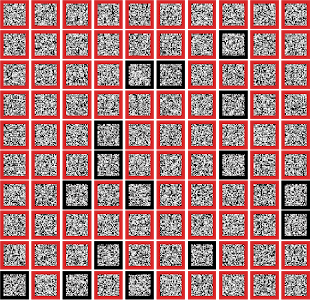
\includegraphics[width=0.9\textwidth]{images/Motivation/pred_noise.png}
    \caption{A model trained to recognize MNIST digits often makes strong predictions over random noise. For each red square, this typical model's softmax output gives over $0.5$ confidence in one of the ten digits, i.e., makes a confident prediction that digit is present in the random image.}
    \label{fig:mot-pred-noise}
\end{figure}
The curse of dimensionality refers to many unintuitive phenomena that arise when analyzing data in high-dimensional spaces, see Zimek et al. 2012 \cite{zimek2012survey}. Notably, distances become hard for humans to visualize. Figure \ref{fig:mot-dist} gives a simplistic example. Other commonly referenced unintuitive phenomena are that high-dimensional spheres have most of their volume concentrated near their surface, and that high-dimensional data sets become easier to linearly separate, see Beyer et al. 1999 \cite{beyer1999nearest}.
\begin{figure}[!t]
    \centering
    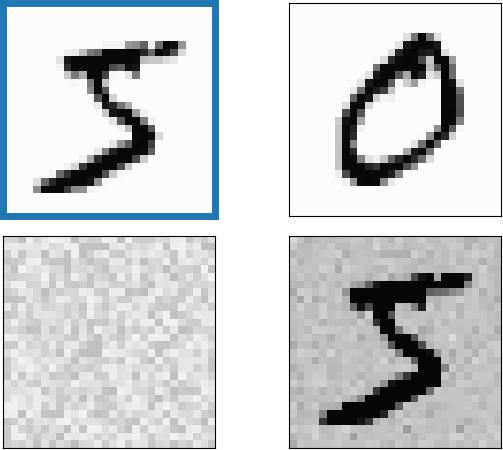
\includegraphics[width=0.9\textwidth]{images/Motivation/motivation-distances.png}
    \caption{Three distinct images that all have the same Euclidean distance to the image in the blue box. Human perception doesn't always align with mathematical definitions.}
    \label{fig:mot-dist}
\end{figure}

The combination of the piece-wise linearity of neural networks with the various unintuitive curse of dimensionality phenomena lead to various unexpected behaviors of neural networks. For example Szegedy et al. 2013 \cite{szegedy2013intriguing} showed that the boundaries between the various classes in the hyper-space (as predicted by a neural network) are often linear and that most real inputs are close distance-wise to every boundary. Figure \ref{fig:mot-bounds} shows an example of this behavior.
\begin{figure}[!t]
    \centering
    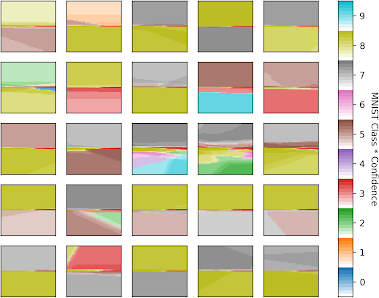
\includegraphics[width=0.9\textwidth]{images/Motivation/boundaries.png}
    \caption{What this simple MNIST model predicts when linearly interpolating between two images. Each pixel in these plots shows the class predicted for an interpolated input MNIST image. The centre-leftmost pixel and centre-rightmost pixel correspond to two images pulled from the data in classes 8 (yellow) and 3 (red), respectively. Left-right movement along the center corresponds to linear interpolation of the two images. Each vertical axis corresponds to movement along a different random vector orthogonal to the left-right image-to-image vector. Each color corresponds to an MNIST class prediction. Surprisingly, while the two images are correctly classified as 8 and 3 respectively, orthogonal movement almost always leads to a different class. An analogy would be: walking in a straight line from Paris to Berlin predictably takes you from France to Germany, but any step left or right of that straight line always lands outside of France or Germany. This image is revisited in Section \ref{Observations}}
    \label{fig:mot-bounds}
\end{figure}

These intuitions motivate the definition of the Finite Gaussian Neuron (in Section \ref{Definition of the FGN}), as a combination of a classical neuron with a Gaussian function of effectively finite support. 


\section{Related Work}
% \subsection{Fast Gradient Sign Method}
% \subsection{Adversarial Training}
Goodfellow et al. 2015 \cite{goodfellow2015explaining} introduce adversarial attacks via the Fast Gradient Sign Method (FGSM). They show that continuous retraining of the model using adversarial examples protects the model from attacks. This adversarial training method however is computationally expensive as it requires both creating new adversarial examples after each training epoch and continuously retraining the model with a growing dataset. They also show that adversarial training based on the FGSM attack does not necessarily protect against other adversarial attacks.
\newpage % pure aesthetics 

Pushing adversarial training further, Madry et al. 2019 \cite{madry2019deep} show that the Projected Gradient Descent (PGD) attack provides adversarial examples that may well generalize to other gradient based attacks. However this potential universal robustness again first-order attacks requires larger networks. In addition, PGD, as an iterated FGSM attack, is especially computationally expensive.

%\subsection{Distillation}
Another proposed defense against adversarial attacks is Distillation, proposed by Papernot et al. 2016 \cite{Papernot2016DistillationAA}. Originally designed as a method to reduce the size of DNNs by transferring knowledge from larger to smaller networks. Distillation works by training a large network, then using the output prediction vectors as soft-labels to train a smaller network, encoding class similarities in the soft-labels. Instead of aiming to reduce model size, the authors show that retraining the same model on the soft-labels provides defense against adversarial attacks by making the network less sensitive to small changes over the input, and requiring a higher average minimum
number of features to be modified in order to create adversarial examples. Similarly to adversarial retraining, distillation requires additional computation to generate the soft-labels and retrain the model.

% \subsection{Radial Basis Function Networks}
Radial Basis Function (RBF) networks have also been explored as a more intrinsic defense against rubbish data and adversarial attacks \cite{moody1989fast, chenou2019radial,zadeh2018deeprbf} and in fact are similar in many ways to the FGN networks. However they have not become as popular as other deep neural networks techniques, perhaps due to their complexity. The RBF architecture doesn't easily generalize to multiple layers, and requires pre-processing work to properly place the prototypes.


\chapter{The Finite Gaussian Neuron}
A classical artificial neuron's output $y_c$ is defined by: 
%%%
\begin{align}
y_{c} &= \varphi(\ell) \label{eq:varphi} \\
\ell &= \sum_{i}w_i x_i \label{eq:ell}
\end{align}
%%%
with $\ell$ being the linear component defined by a linear combination of the inputs $x_i$ and associated weights $w_i$, and with $\varphi$ being the non-linear activation function required by the universal approximator theorem by Cybenko and Hornik in 1089 \cite{cybenko1989approximation, hornik1989multilayer}. The bias term can be implicitly included as an extra input with value 1 or explicitly included. Figure \ref{fig:classic-neuron} gives a visualization of this classical neuron. 
\begin{figure}[!h]
    \centering
    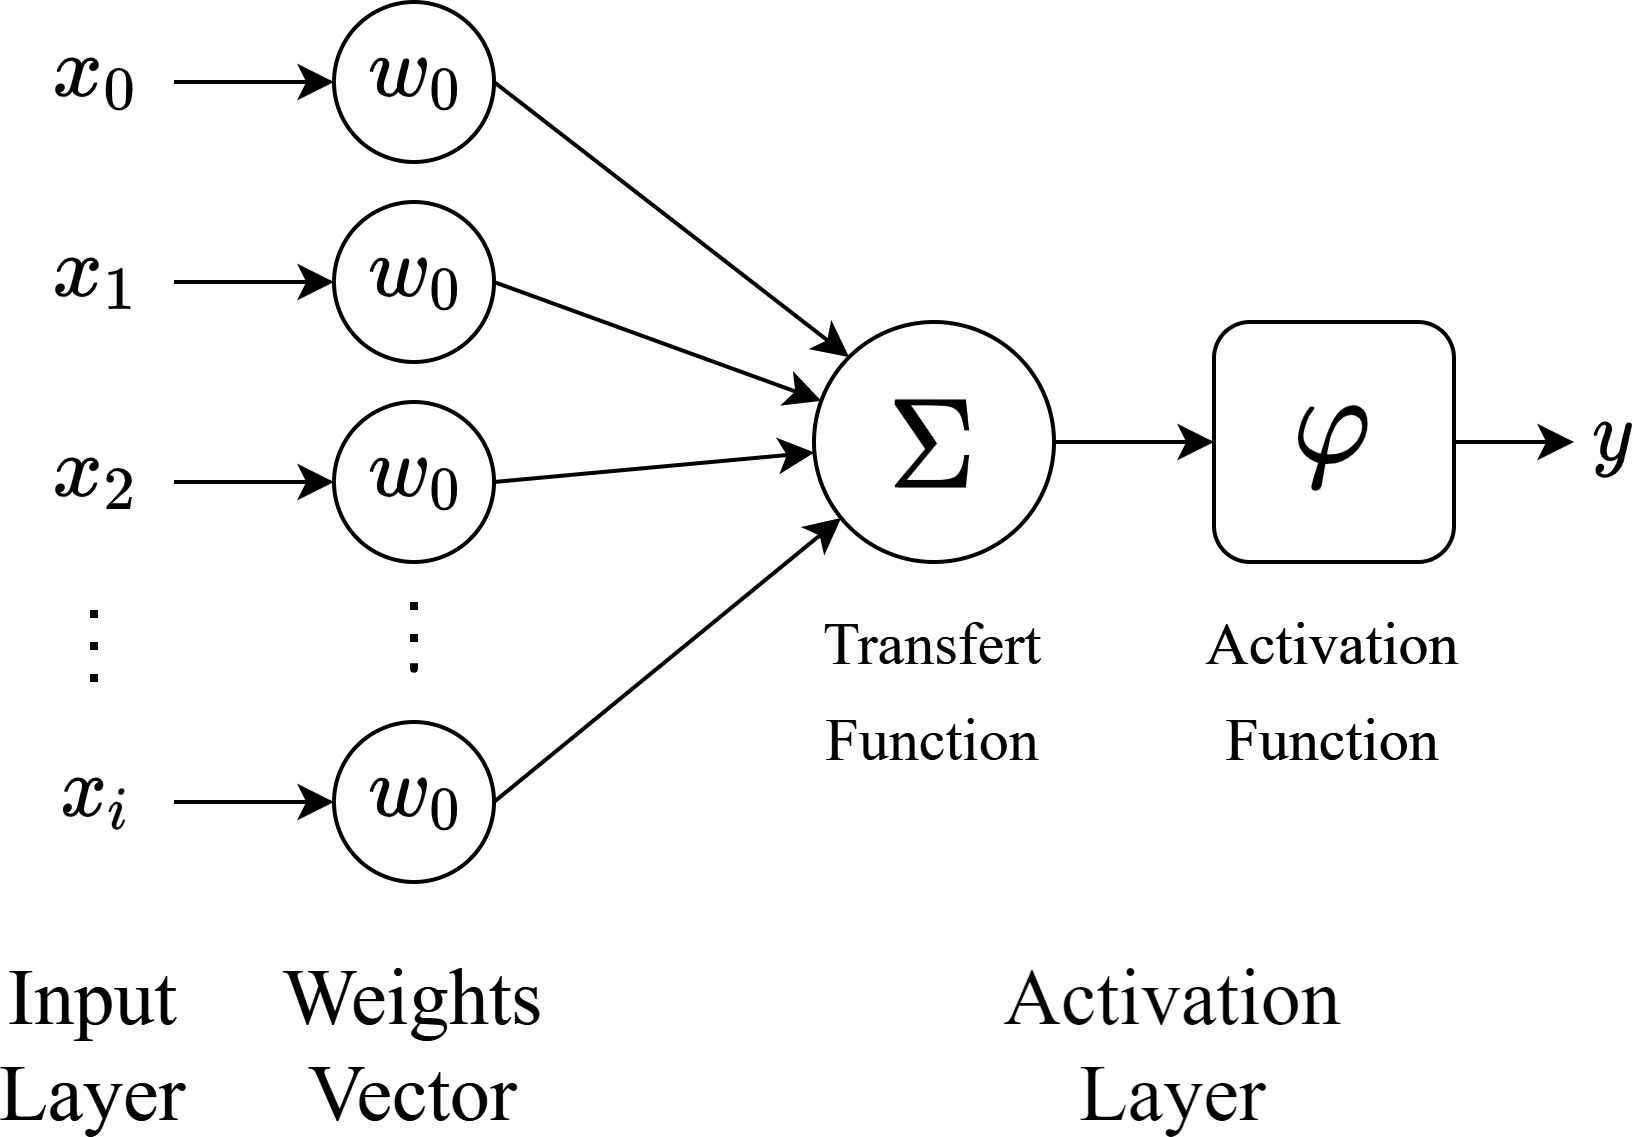
\includegraphics[width=0.9\textwidth]{images/classic-neuron.png}
    \caption{A classical representation of the artificial neuron.}
    \label{fig:classic-neuron}
\end{figure}
\newline %explicitly to prevent the FGN definition from being split

\section{Definition of the FGN} \label{Definition of the FGN}
I introduce the Finite Gaussian Neuron (FGN) as a combination of the classical neuron's activity with a Gaussian activity that limits the effective support of the neuron. Explicitly, the FGN's output $y_f$ is given by:
%%%
\begin{align}
y_{f} &= \varphi(\ell) * g \\
g &= e^{\frac{-1}{\sigma^2}\sum_{i}(x_i-c_i)^2}
\end{align}
%%%
with $\ell$ and $\varphi$ the same as in Equations~\eqref{eq:ell} and \eqref{eq:varphi}, i.e., the linear component and non-linear activation function respectively; and with $g$ the new Gaussian component, defined by centers $c_i$ that position the neuron in the input hyperspace, and variance $\sigma$ that prevents the neuron's activity from covering the entire input space. If inputs are far away from the center, relative to the variance $\sigma$, then the Gaussian component $g$ approaches value zero and the FGN's output activity will approach zero as well, thus limiting the effective support of neurons to a limited zone of the input hyperspace. Figure \ref{fig:gaussian-comp} gives a visualization of the new Gaussian component $g$.
\begin{figure}[!t]
    \centering
    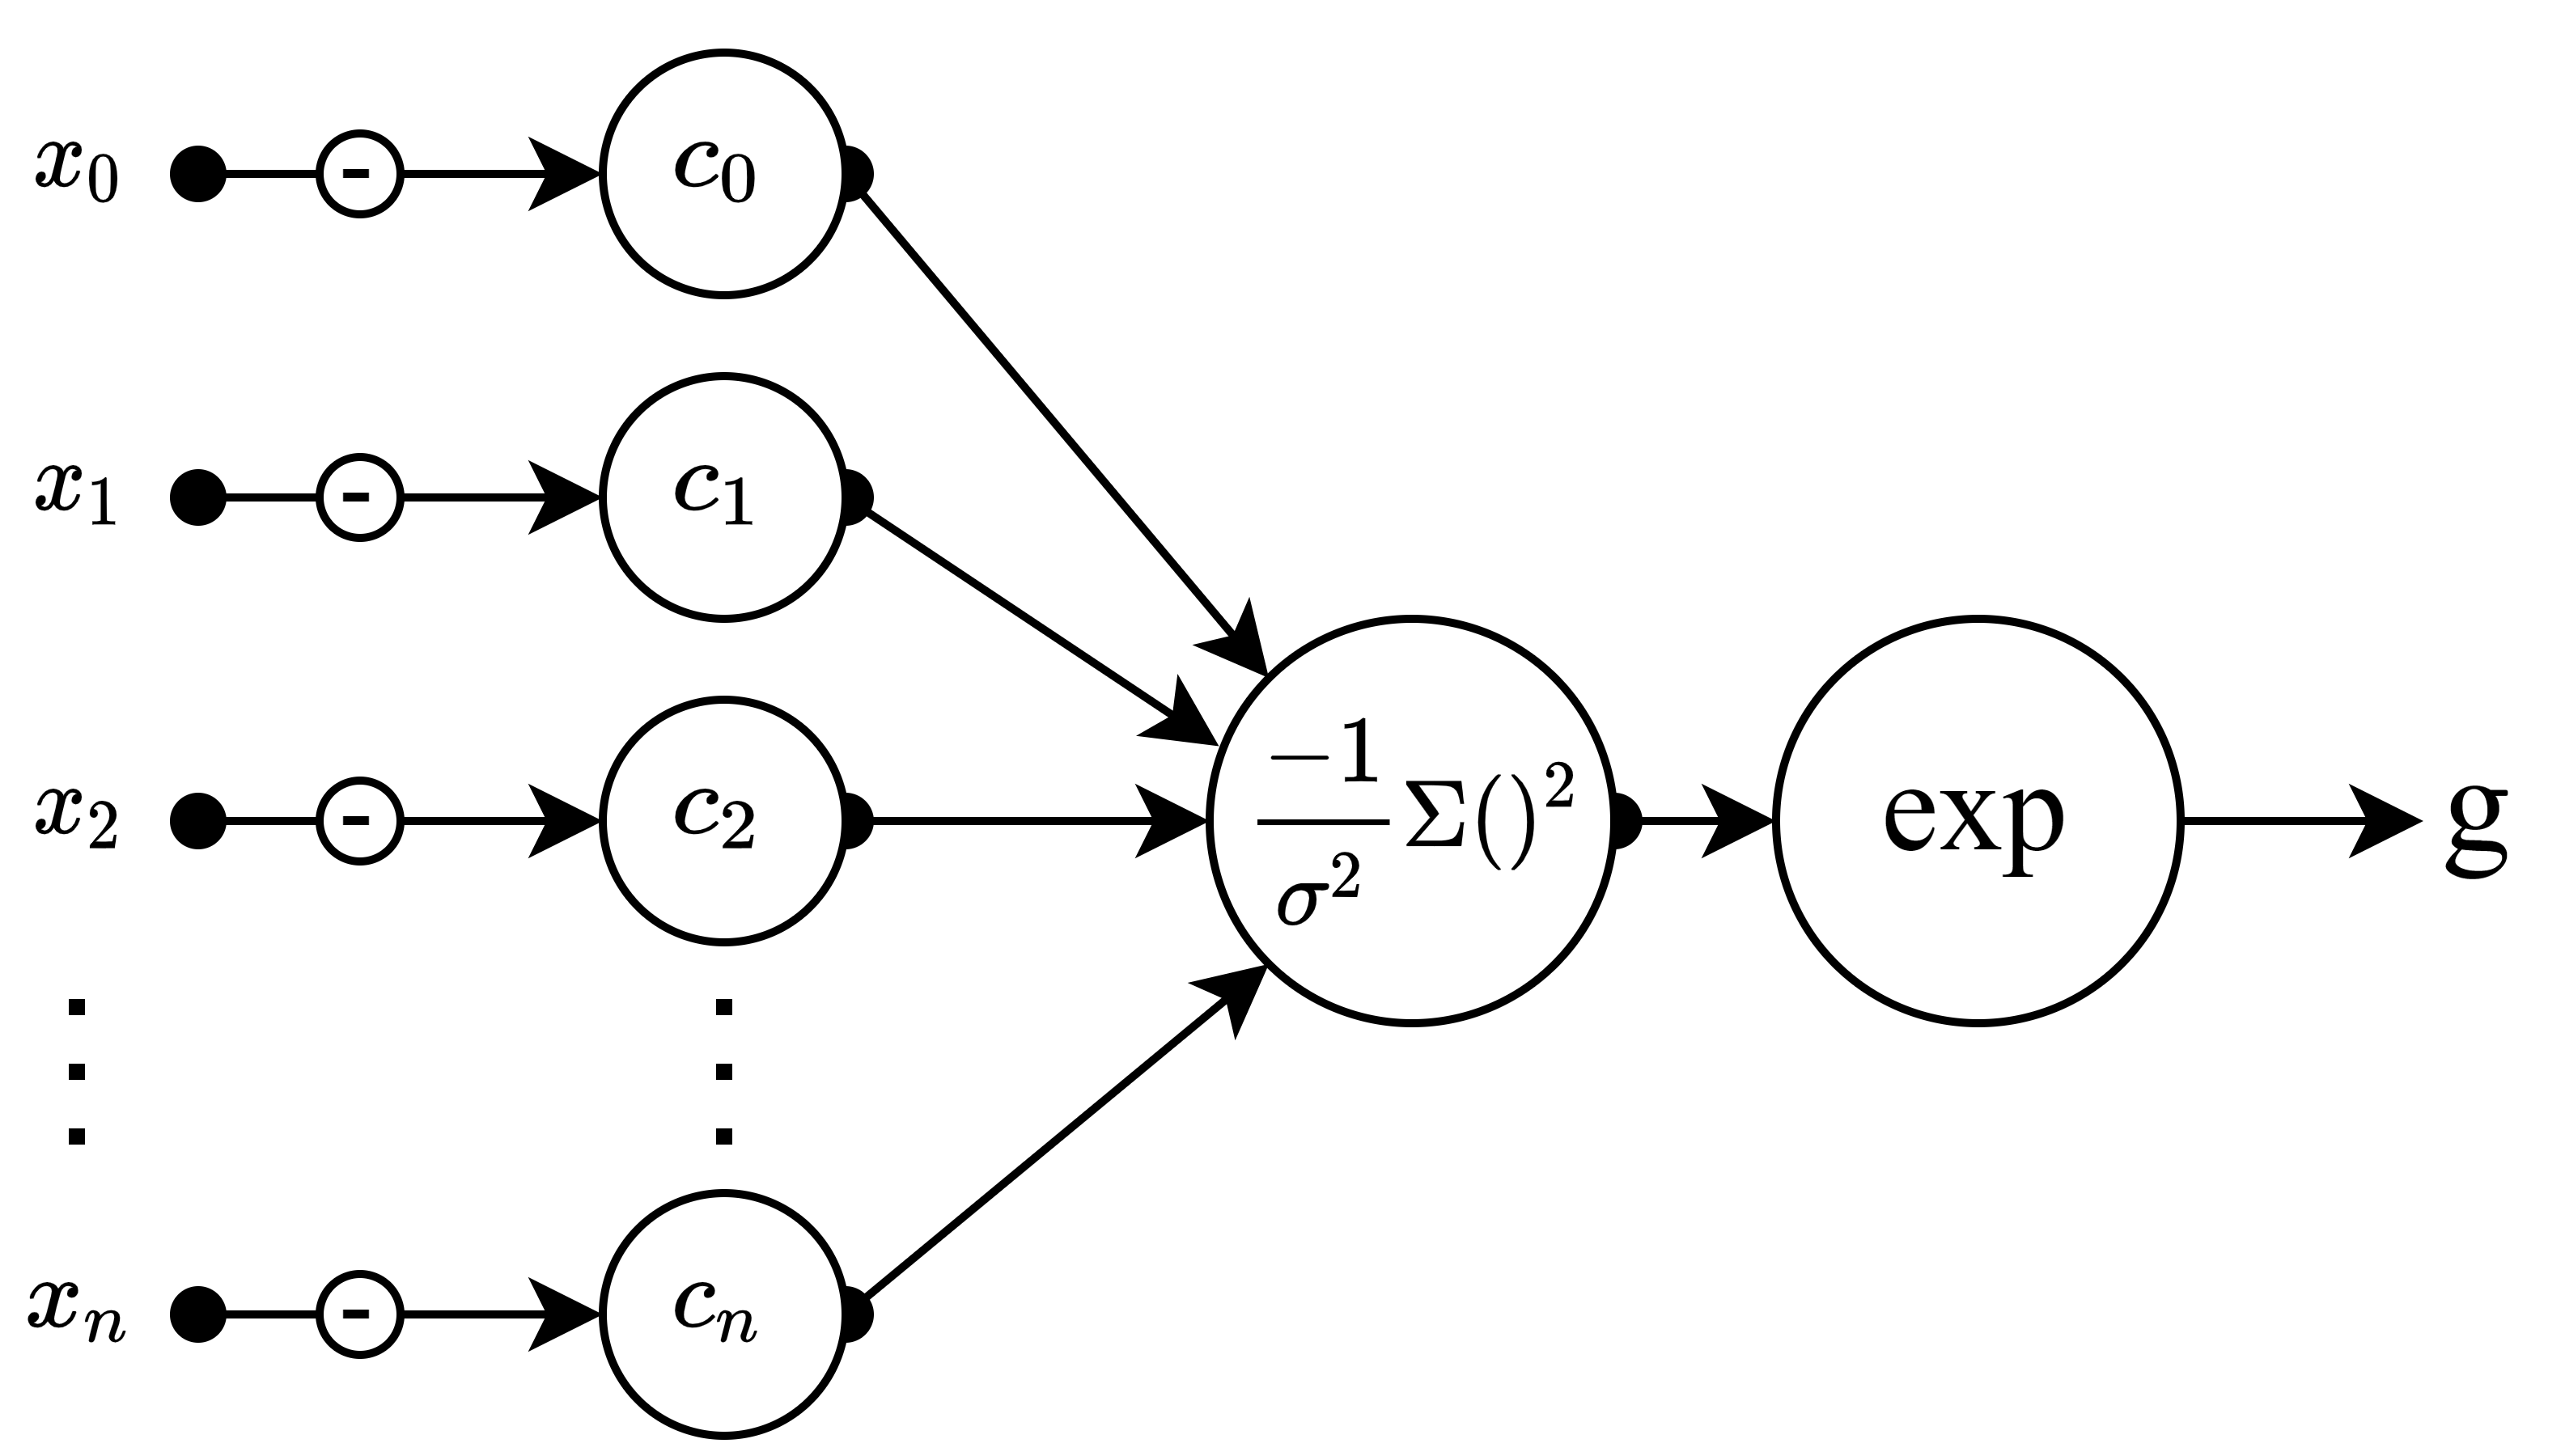
\includegraphics[width=0.9\textwidth]{images/fgn-gaussian-component.png}
    \caption{The Gaussian component of an FGN.}
    \label{fig:gaussian-comp}
\end{figure}
% visuals

The following figures (\ref{fig:classic-heatmap}, \ref{fig:fgn-heatmap}) show the difference in behavior between the classical neuron architecture and the FGN architecture, for an arbitrary neuron, over a two dimensional input space.
\begin{figure}[!t]
    \centering
    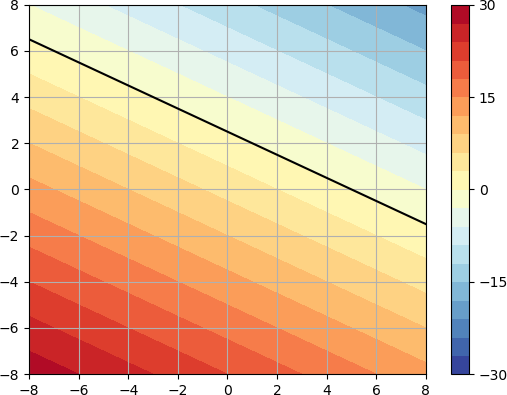
\includegraphics[width=0.49\textwidth]{images/2D Activity/2d-linear-activity-cropped.png}
    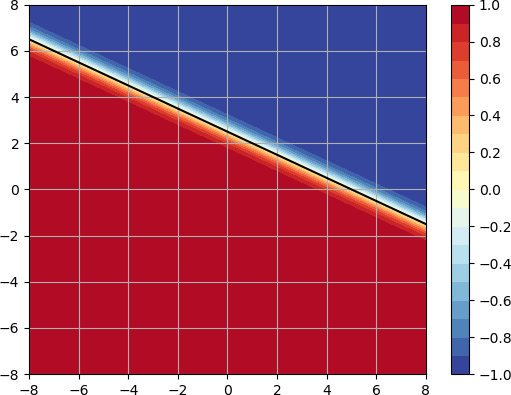
\includegraphics[width=0.49\textwidth]{images/2D Activity/2d-classic-activity-cropped.png}
    \caption{On the left, the $\ell = \sum_{i}w_i x_i$ linear component of the classical neuron with arbitrary weights, shown as an activity heatmap over a 2D input space. On the right the same neuron's output $y_c = \tanh(\ell)$  after the linear component is passed through the typical $tanh$ non-linear activation function. The black line shows where the heatmap value is zero.}
    \label{fig:classic-heatmap}
\end{figure}
\begin{figure}[!t]
    \centering
    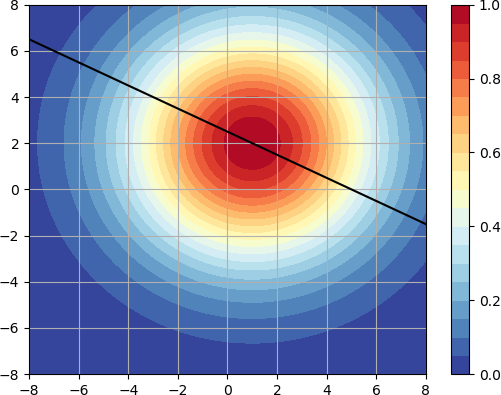
\includegraphics[width=0.49\textwidth]{images/2D Activity/2d-gaussian-activity-cropped.png}
    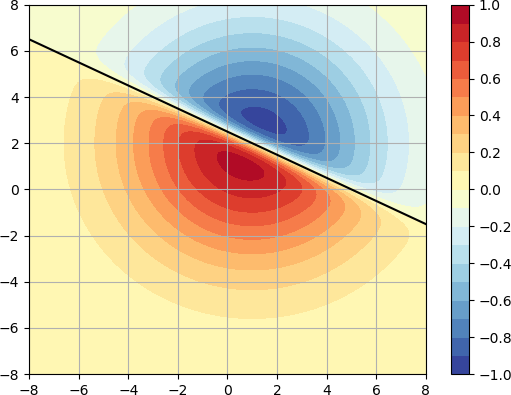
\includegraphics[width=0.49\textwidth]{images/2D Activity/2d-fgn-activity-cropped.png}
    \caption{On the left, the Gaussian component $g = e^{\frac{-1}{\sigma^2}\sum_{i}(x_i-c_i)^2}$ of the FGN architecture with arbitrary centers and variance, shown as an activity heatmap over a 2D input space. The line in this image is only for comparison with the other images. On the right, the FGN's output $y_f = \tanh(\ell) * g$ combining the output of the classical neuron with the Gaussian component. Note the limited effective support of the FGN's activity.}
    \label{fig:fgn-heatmap}
\end{figure}

% desired behavior
The desired outcome of defining the FGN in this way is to restrict the activity of the neural network to regions of the input hyperspace where data has been observed during training, while making no predictions over regions never observed. And, if this works as intended, the FGN networks will be more resistant to adversarial examples compared to classical networks.

\section{Classic Neuron Conversion to FGN}
One important property of the FGN is that existing networks using the classical neuron can be converted to the FGN architecture without changing the network's behavior over a given dataset, and without heavy computation. This is done by converting each classical neuron in the original network to an FGN with identical weight vector $W$ and large variance $\sigma$. Figure \ref{fig:matching} illustrates this property.
\begin{figure}[!t]
    \centering
    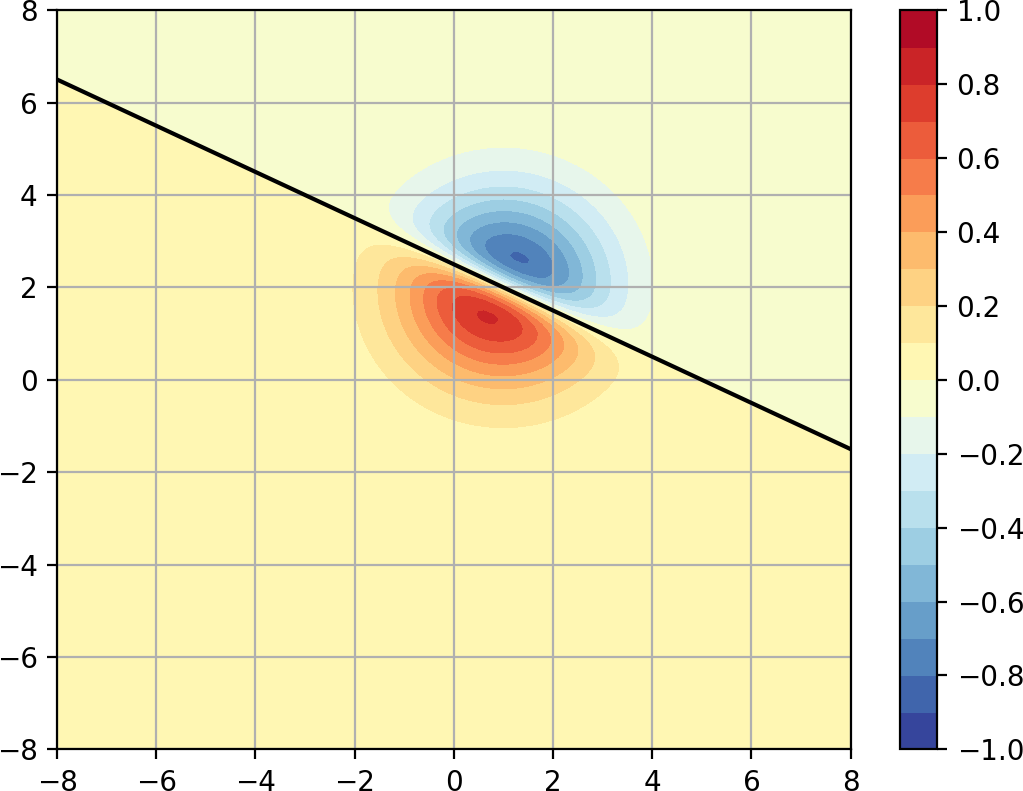
\includegraphics[width=0.32\textwidth]{images/Matching-behavior/sigma-2-cropped.png}
    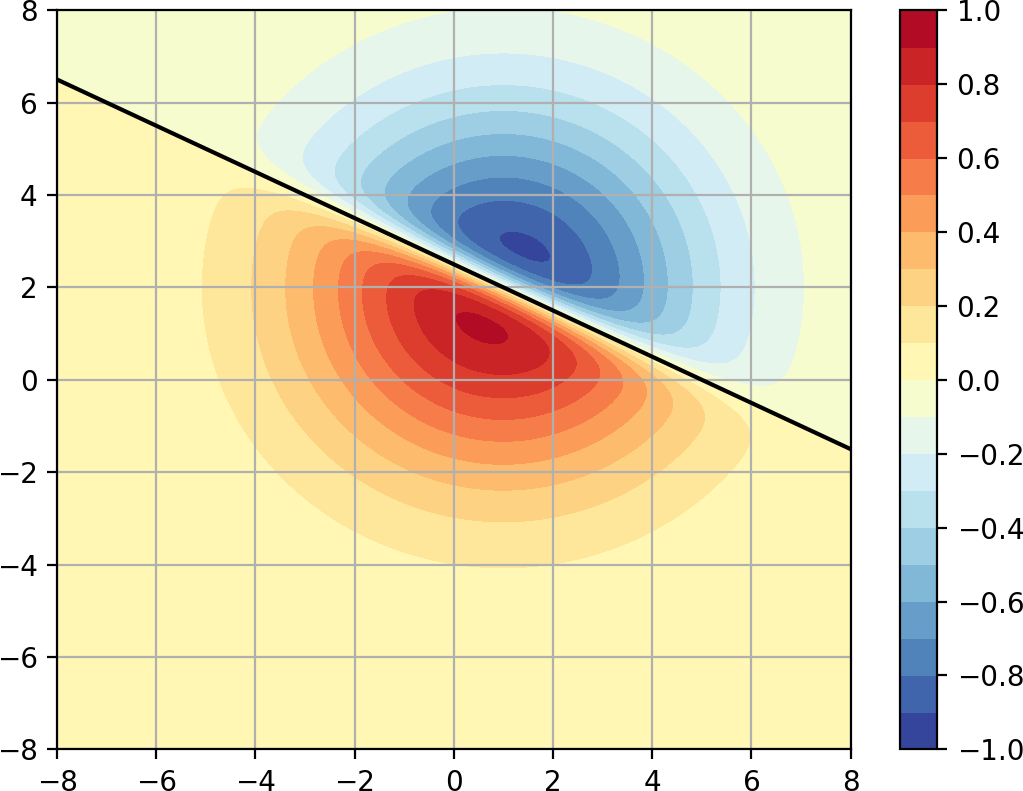
\includegraphics[width=0.32\textwidth]{images/Matching-behavior/sigma-3-cropped.png}
    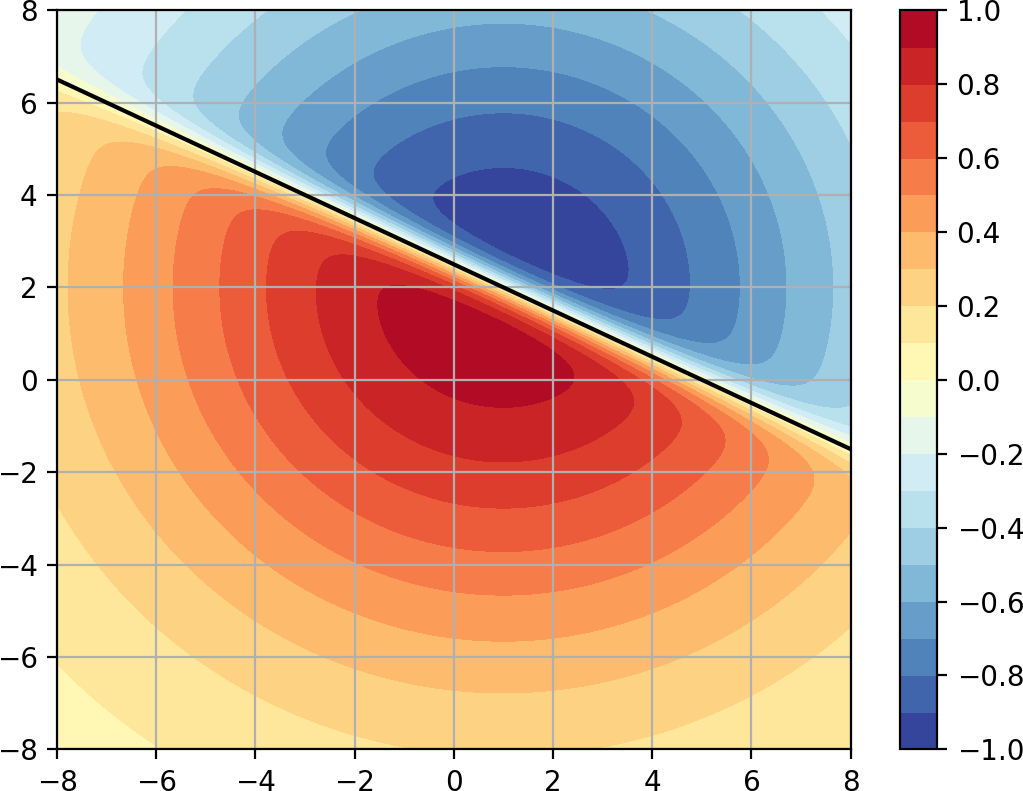
\includegraphics[width=0.32\textwidth]{images/Matching-behavior/sigma-4-cropped.png}
    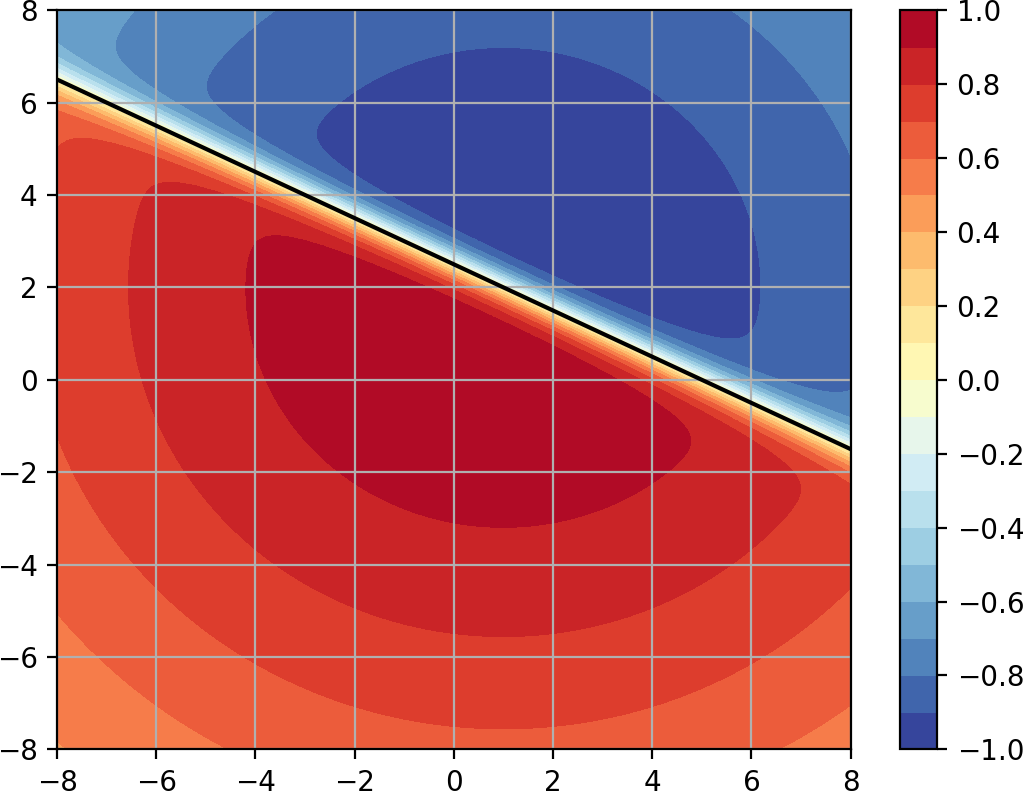
\includegraphics[width=0.32\textwidth]{images/Matching-behavior/sigma-5-cropped.png}
    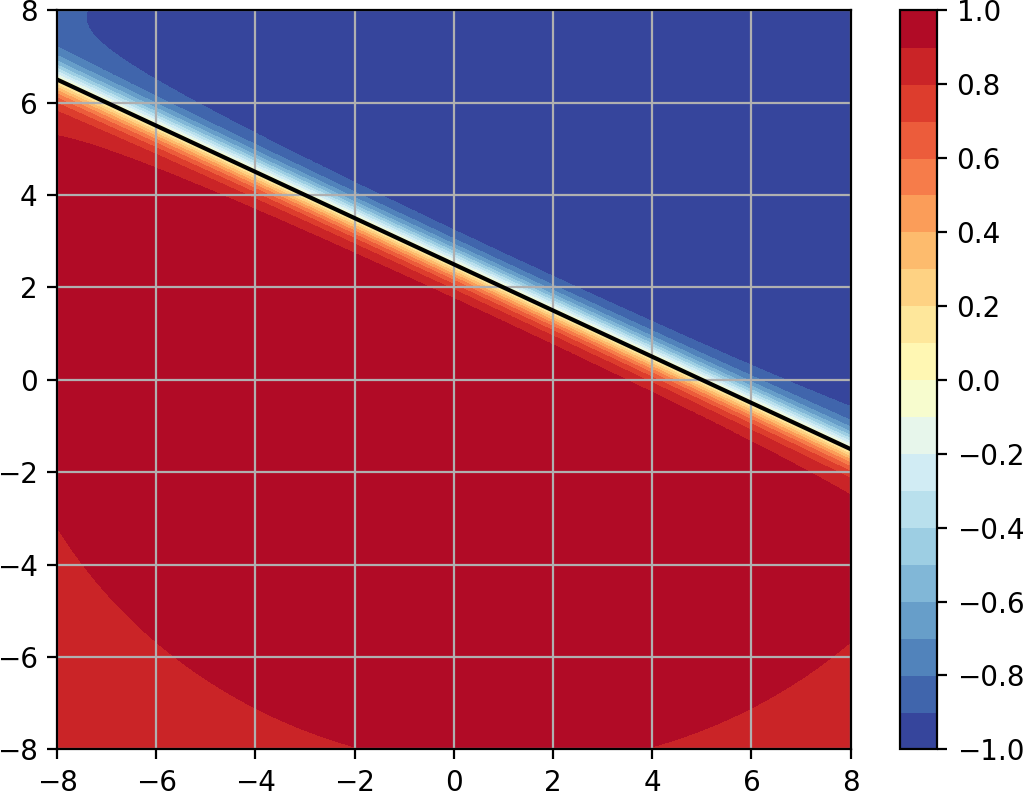
\includegraphics[width=0.32\textwidth]{images/Matching-behavior/sigma-6-cropped.png}
    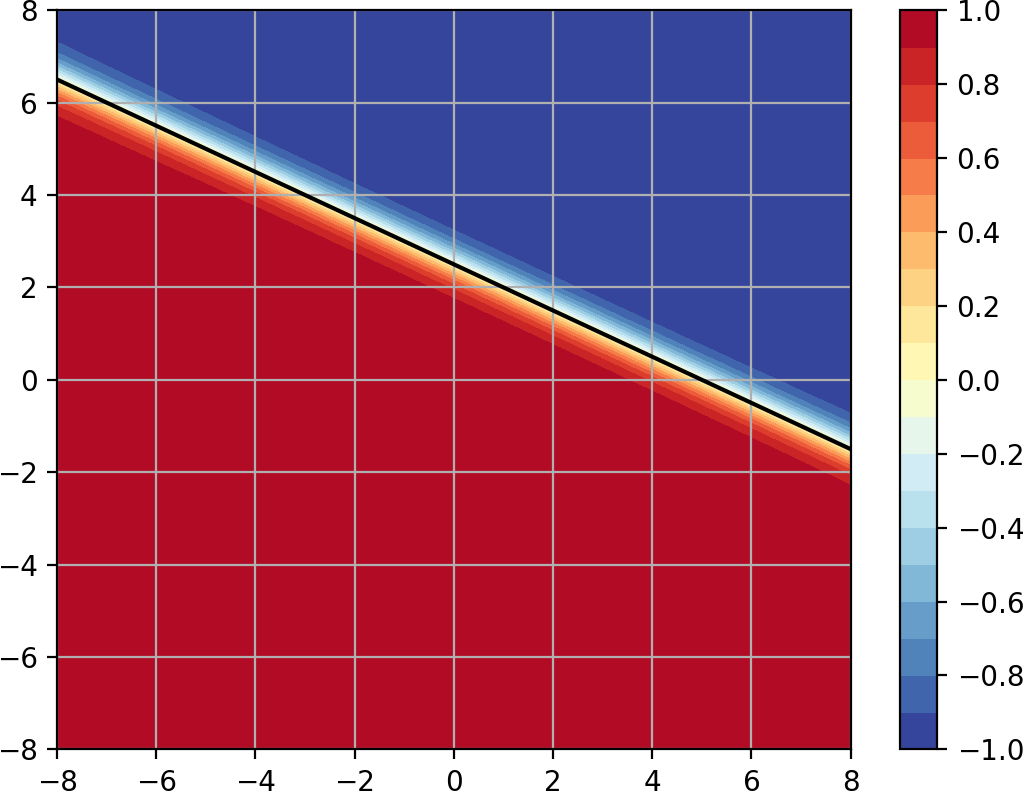
\includegraphics[width=0.32\textwidth]{images/Matching-behavior/sigma-7-cropped.png}
    \caption{Illustration showing that increasing an FGN's variance $\sigma$ (smallest top-left, largest bottom-right) leads to behavior identical to that of classical neuron with the same weights $W$. Note how the final picture is indistinguishable that shown in figure \ref{fig:classic-heatmap}. }
    \label{fig:matching}
\end{figure}

Converting a classical neuron to an FGN involves defining two new parameters, the variance $\sigma$ and the centers $c_i$. For any given dataset, there will be a unique $C=[c_i]$ that allows for minimum valued variance while not changing the behavior over this dataset. Finding this center is not trivial, and the topic of future research. Currently, conversion is done by setting the center $C$ to be the point on the zero-output line (defined by the neuron weights $W$) closest to the origin, and empirically searching for a variance $\sigma$ large enough.

\section{Training the FGN}
Training the FGN is done much the same way as the classical neuron: we find parameters of the FGN that locally minimize a loss function using the back-propagation algorithm. So far, experiments have not shown any specific loss function (Mean-Squared Error, Cross-Entropy, etc...) or gradient descent optimizer algorithm (Adam, RMSprop, etc...) to perform any differently on FGNs versus classical neurons.

Since one of the goals of the FGN is to limit the activity far from the data, we add a regularization term $\lambda$ to the loss function $\mathcal{L} $ to add pressure to minimize the variance $\sigma$ during training. $\lambda$ becomes a hyper-parameter of the neuron to tune to the task like any other hyper-parameter.
%%%
\begin{align}
\mathcal{L}  = \tilde{\mathcal{L} } + \lambda\sigma^2
\end{align}
%%%
The precise gradients depend on the loss $\mathcal{L}$ and non-linear activation $\varphi$ functions chosen, but the partial derivatives of the FGN output $y$ for an input $x_i$  are:
\begin{align}
    \text{Weights:\quad} \frac{\partial y}{\partial w_i} &=  x_i \varphi'(\ell) * g  \\[1em]
    \text{Centers:\quad} \frac{\partial y}{\partial c_i} &= \varphi(\ell) * \frac{2(x_i-c_i)}{\sigma^2} * g \\[1em]
    \text{Sigmas:\quad} \frac{\partial y}{\partial \sigma} &= \varphi(\ell) * \frac{2\sum_{i}(x_i-c_i)^2}{\sigma^3}* g
    % \text{(Reminder:\quad} y &=  \varphi(\ell)*g = \tanh(\sum_i x_i w_i) * e^{\frac{-1}{\sigma^2}\sum_{i}(x_i-c_i)^2} )
\end{align}

The changes to each of the parameters all depend in part on the Gaussian component $g$. In particular they all need it to be non-zero or they will not change. This shows that the FGN can only learn when the input is close to the neuron centers $c_i$ relative to the variance $\sigma$. Proper initialization is thus important, to ensure that the FGN variance and centers cover the data, else the gradients will be non-existent.

As a sanity check, I verified that a single FGN is able to be trained to properly classify a two dimensional linearly separable toy dataset, show in figure \ref{fig:single-fgn-1}. The following figures \ref{fig:single-fgn-2}, \ref{fig:single-fgn-3} show the FGN's weights $W$, centers $c_i$ and variance $\sigma$ adapting to fit the data.
\begin{figure}[!b]
    \centering
    \hspace{0.0\textwidth}
    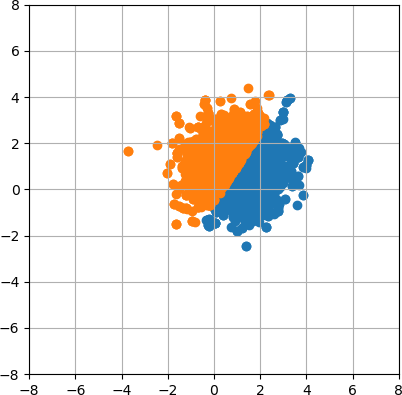
\includegraphics[width=0.405\textwidth]{images/2D-single-neuron/2d-easy-data-cropped.png}
    \hspace{0.04\textwidth}
    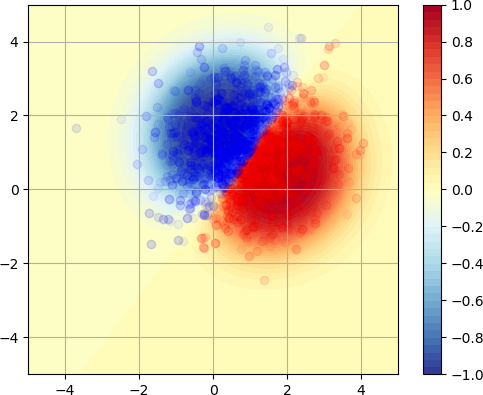
\includegraphics[width=0.49\textwidth]{images/2D-single-neuron/2d-easy-trained-activity-cropped.png}
    \caption{The 2D linearly separable toy data centered on $(1,1)$, and the activity of the FGN over the space after training with MSE loss function, $\lambda=0.01$ variance $\sigma$ regularization term, Adam optimizer with $lr=0.05$.}
    \label{fig:single-fgn-1}
\end{figure}
\begin{figure}[!b]
    \centering
    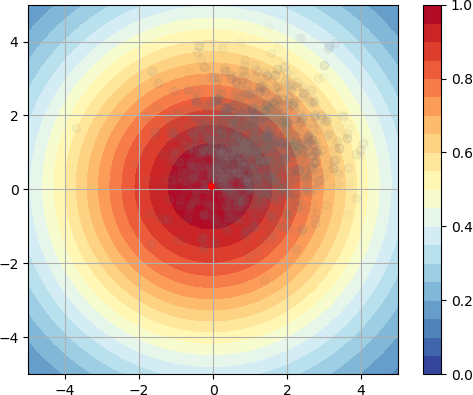
\includegraphics[width=0.49\textwidth ]{images/2D-single-neuron/2d-easy-initialg-cropped.png}
    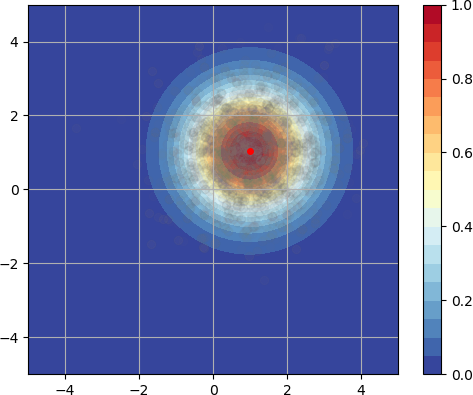
\includegraphics[width=0.49\textwidth]{images/2D-single-neuron/2d-easy-trainedg-cropped.png}
    \caption{The FGN's Gaussian component $g$ activity over the 2D space pre and post training. Initially centered on the origin $(0,0)$ with variance $\sigma=5$, after training the Gaussian component is centered on the data and the variance has shrunk such that space far from the data has $g=0$ activity.}
    \label{fig:single-fgn-2}
\end{figure}\\
\begin{figure}[!t]
    \centering
    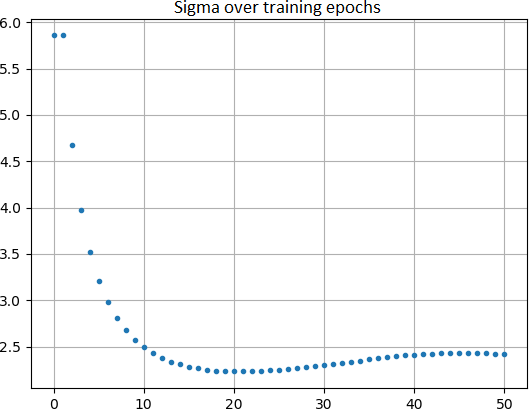
\includegraphics[width=0.49\textwidth,height=6.35cm]{images/2D-single-neuron/2d-easy-sigma-training-cropped.png}
    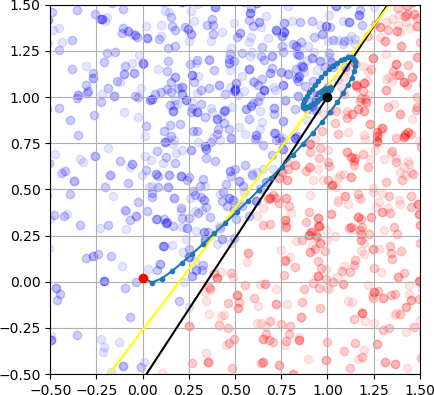
\includegraphics[width=0.49\textwidth]{images/2D-single-neuron/2d-easy-center-path-cropped.png}
    \caption{Evolution of the FGN's variance $\sigma$ and center position during training. On the left, pressured by the loss function's regularizer term $\lambda$,  the variance $\sigma$ shrinks as much as possible while still fitting the data.  On the right, the dotted blue line shows the FGN center's path during training, starting from the red dot in $(0,0)$ and moving towards the theoretically optimal center $(1,1)$ (black dot). The black line is the class border and the yellow line is the FGN's predicted border, given by the weights $W$.}
    \label{fig:single-fgn-3}
\end{figure}

\section{Alternative Implementations}
There are several implementation alternatives that may improve the FGN's performance on specific tasks.

An FGN built to match the behavior of a classical neuron will define the bias term of the linear component $\ell$ by the centers of the FGN, so that the line of zero activity for the linear component passes through the center. This isn't strictly needed when retraining the FGN or when training from scratch. Figure \ref{fig:decoupled} is an example of an FGN with decoupled bias and centers in two dimensional input space. All the experiments performed in later sections were done with decoupled bias and centers.
\begin{figure}[!t]
    \centering
    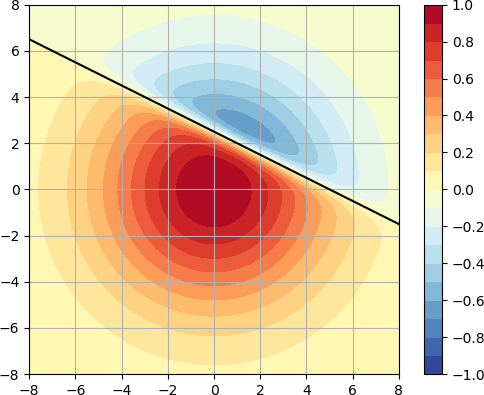
\includegraphics[width=0.66\textwidth]{images/2D-Decoupled/var-decoupled-center-activity-cropped.png}
    \caption{Activity of an FGN with a decoupled bias and centers.}
    \label{fig:decoupled}
\end{figure}

Since distances in higher dimensions are harder to grasp, various norms for the Gaussian component $g$ were considered over the Euclidean norm.
\begin{align}
    g = e^{\frac{-1}{\sigma^2}\lVert x_i-c_i \lVert_p }
\end{align}
Figure \ref{fig:norms} shows how changing the ordinal $p$ of the norm affects the FGN's output, visualized over a two dimensional input space. Cursory experiments have not shown any differences in FGN performance between the various $p$-norms, and the Euclidean norm was used.
\begin{figure}[!t]
    \centering
    \begin{subfigure}[t]{0.32\textwidth}
        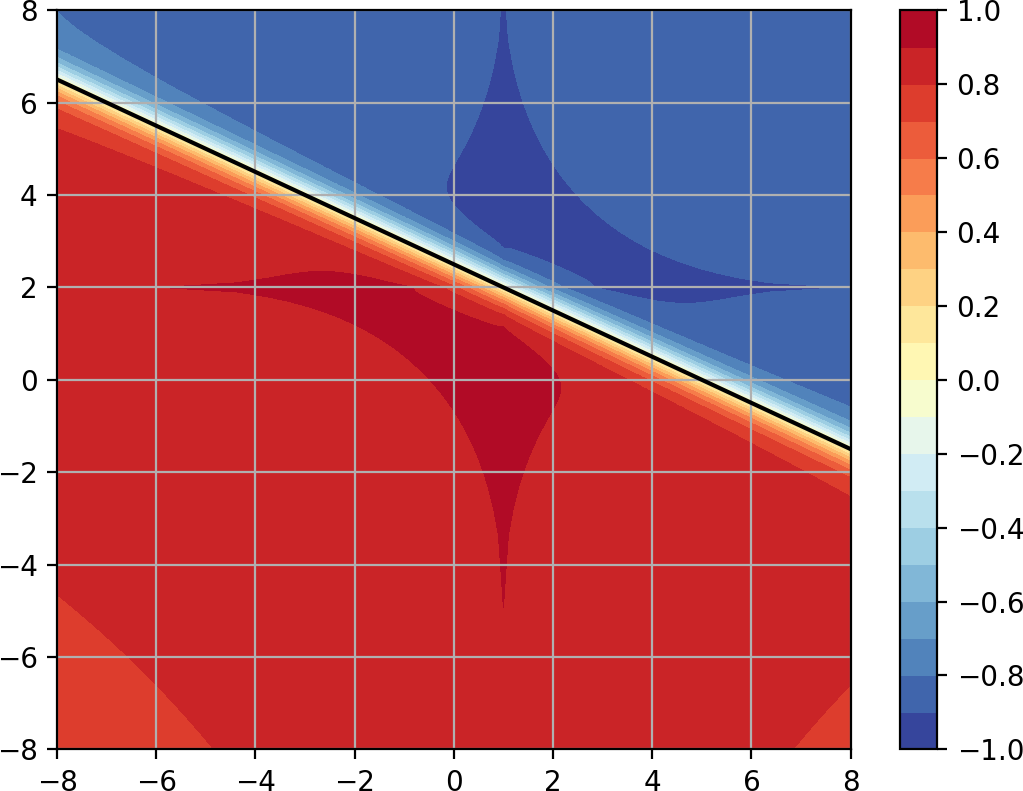
\includegraphics[width=\textwidth]{images/Variants-Norms/ord0.5-cropped.png}
        \caption*{$p=0.5$}
    \end{subfigure}
    \begin{subfigure}[t]{0.32\textwidth}
        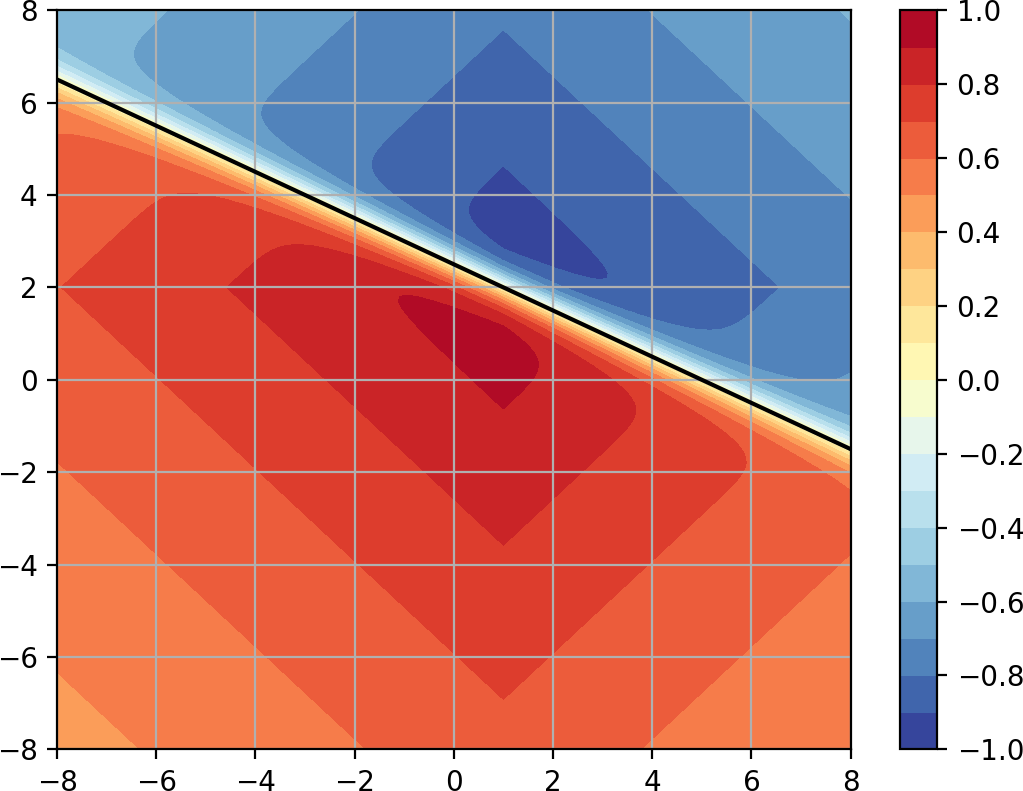
\includegraphics[width=\textwidth]{images/Variants-Norms/ord1-cropped.png}
        \caption*{$p=1.0$}
    \end{subfigure}
    \begin{subfigure}[t]{0.32\textwidth}
        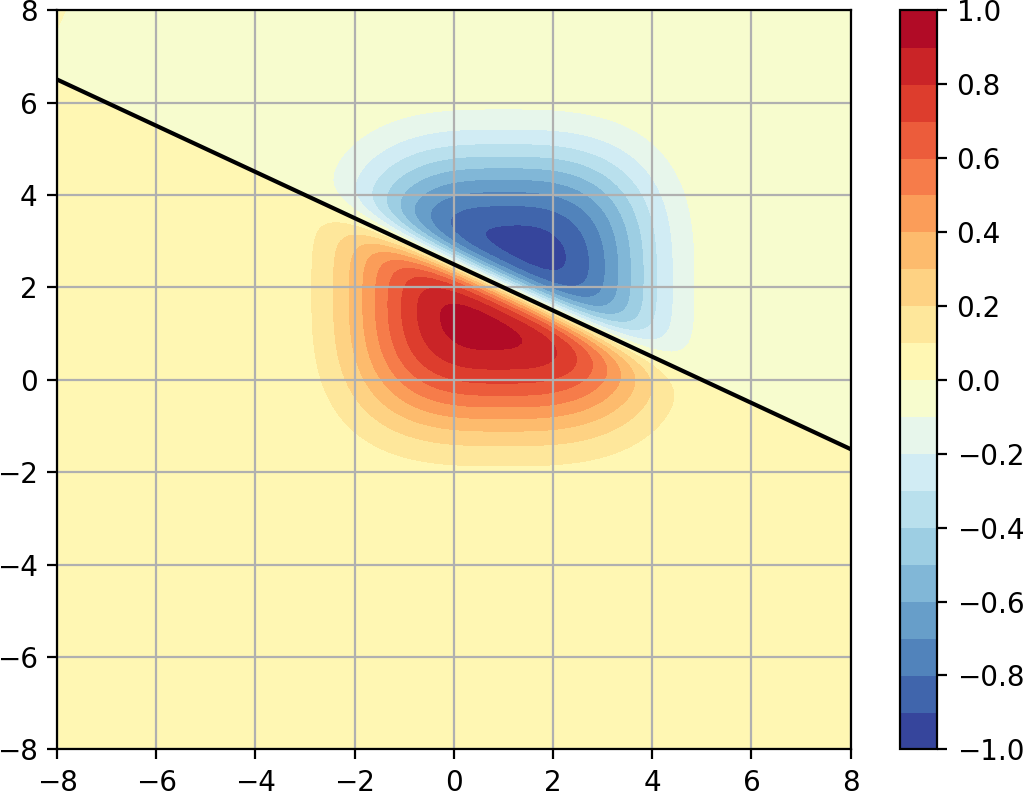
\includegraphics[width=\textwidth]{images/Variants-Norms/ord3-cropped.png}
        \caption*{$p=3.0$}
    \end{subfigure}
    \caption{Examples of how the $p$-norm of the FGN's Gaussian component affects activity.}
    \label{fig:norms}
\end{figure}

The variance term $\sigma$, which defines how large or small the hyper-sphere of activity is for the Gaussian component $g$, can be modified into a matrix $\Sigma$ to stretch and/or rotate the sphere into an ellipse, which gives the FGN a different variance along each of its inputs.

The Gaussian component $g$ then becomes
\begin{align}
    g = e^{-(X-C)^T * \Sigma^{-1} * (X-C)}
\end{align}
with $X=[x_i]$ the inputs vector, $C=[c_i]$ the centers vector and $\Sigma$ the covariance matrix (semi-definite positive). Figure \ref{fig:covars} gives examples of such $\Sigma$ matrices. Note that a full $\Sigma$ matrix has $N^2=$ elements, with $N$ being the number of inputs to the FGN, making the computation of $g$ intractable for any larger problem. A diagonal $\Sigma$ matrix is feasible.
\begin{figure}[!t]
    \centering
    \begin{subfigure}[t]{0.49\textwidth}
        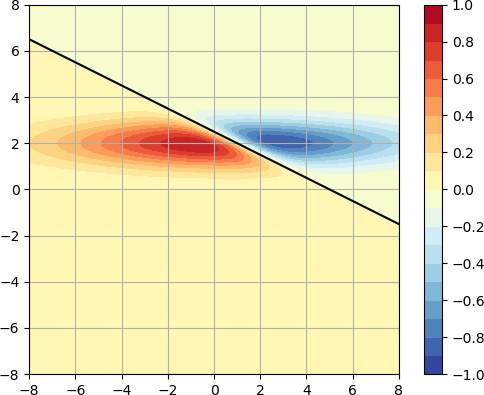
\includegraphics[width=\textwidth]{images/Variants-Diag-Full-Cov/diag_full_activity_cropped.png}
        \caption*{Diagonal $\Sigma$}
    \end{subfigure}
    \begin{subfigure}[t]{0.49\textwidth}
        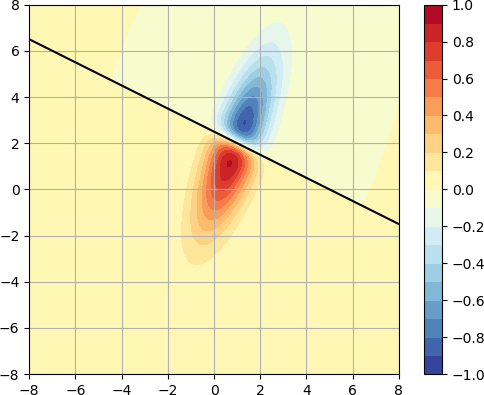
\includegraphics[width=\textwidth]{images/Variants-Diag-Full-Cov/full_full_activity_cropped.png}
        \caption*{Full $\Sigma$}
    \end{subfigure}
    \caption{Examples of how using a covariance $\Sigma$ matrix, rather than a scalar value $\sigma$, allows the FGN to consider changes along one input dimension to be more important than others.}
    \label{fig:covars}
\end{figure}

\section{Multi-Layer FGN Networks}
Extending the FGN architecture to neural networks is straightforward save for one detail: the Gaussian component $g$ of an FGN needs to consider the Gaussian components of its input from the previous layer to be able to propagate out-of-range activities. Without this Gaussian gate, activity far from the data defaults to an arbitrary value, not necessarily to zero as desired. A layer $j$ FGN's output $y$ is given by
\begin{align}
    y =  \varphi(\ell)*g = \varphi(\sum_i x_{i} w_{i}) * g\\
    g = \max(G_{j-1}) * e^{\frac{-1}{\sigma^2}\sum_{i}(x_i-c_i)^2}
\end{align}
With $x_{i}$ and $G_{j-1}$ the previous layer outputs and Gaussian components. For the initial layer, $\max(G_{j-1})$ should be set to $1$. Figure \ref{fig:fgn-layer} illustrates this process.
\begin{figure}[!t]
    \centering
        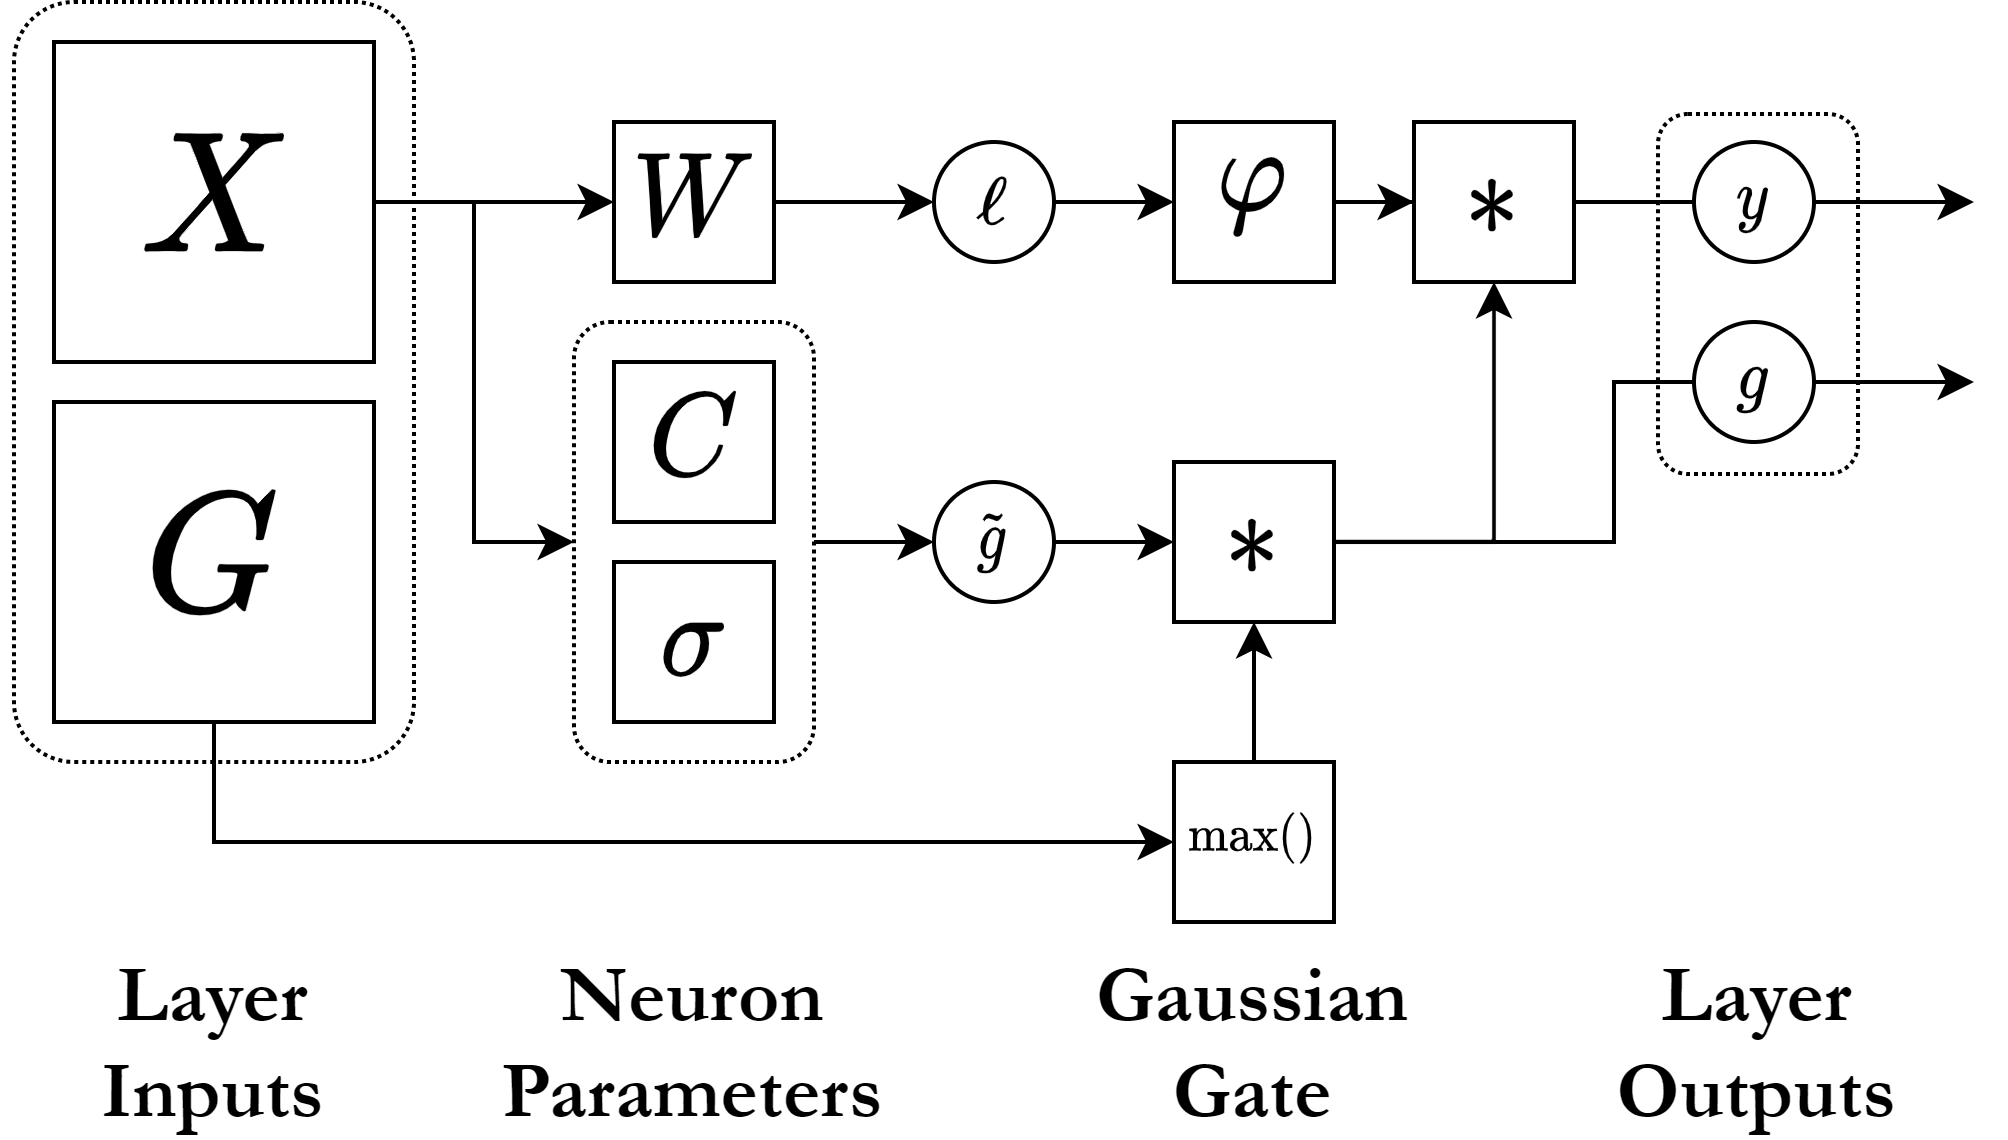
\includegraphics[width=\textwidth]{images/multi-layer-fgn/FGN-Network.png}
    \caption{Illustration of an FGN's output computation when integrated in a neural network. The added Gaussian gate allows for zero activity due to out-of-range inputs to propagate throughout the network. Both $y$ ang $g$ are outputed to the next layer.}
    \label{fig:fgn-layer}
\end{figure}

% toy 2D data
To illustrate the difference in behavior between a neural network built from classical neuron compared to a network built from FGNs, consider the two class, two dimensional, non-linearly separable toy dataset in figure \ref{fig:toy-2d-data}. After training two fully-connected feedforward neural networks, one with FGNs and the other with classical neurons but otherwise identical, figure \ref{fig:toy-2d-activities} shows that, while both networks are able to properly separate the two classes, the FGN network restricts its predictions to zones of the space where the data is present, while the classical network does not. Figure \ref{fig:toy-2d-params} gives additional details on the experiment.

\begin{figure}[!t]
    \centering
        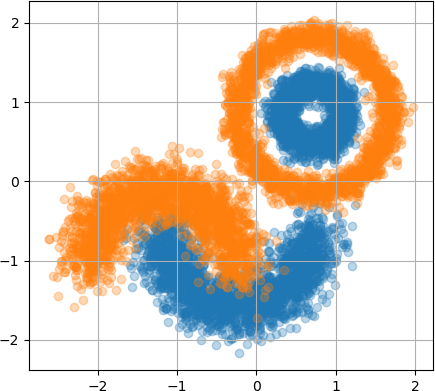
\includegraphics[width=0.66\textwidth]{images/2D-network-toy/2d-toy-data.png}
    \caption{Two class, two dimensional, non-linearly separable toy dataset}
    \label{fig:toy-2d-data}
\end{figure}
\begin{figure}[!t]
    \centering
    \begin{subfigure}[t]{0.49\textwidth}
        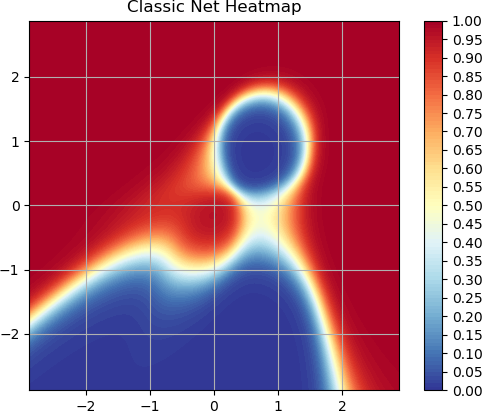
\includegraphics[width=\textwidth]{images/2D-network-toy/classic-heatmap.png}
        % \caption*{}
    \end{subfigure}
    \begin{subfigure}[t]{0.49\textwidth}
        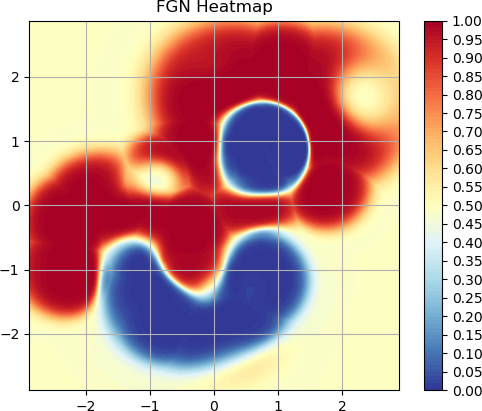
\includegraphics[width=\textwidth]{images/2D-network-toy/fgn-heatmap.png}
        % \caption*{}
    \end{subfigure}
    \caption{Comparison of the activity heatmap between a classical neural network and the same network except using FGNs instead of classical neurons. Both networks separate the data shown in figure \ref{fig:toy-2d-data}, but only the classical network makes predictions far from the data.}
    \label{fig:toy-2d-activities}
\end{figure}
\begin{figure}[!t]
    \centering
    \begin{subfigure}[t]{0.49\textwidth}
        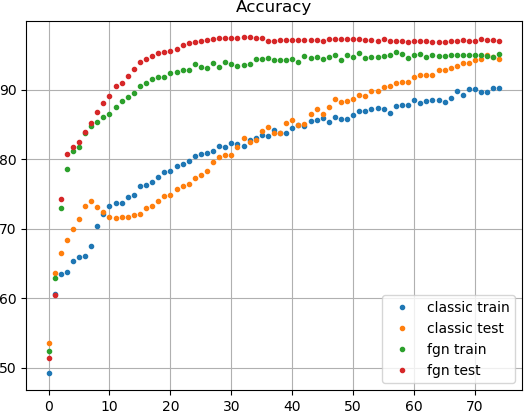
\includegraphics[width=\textwidth]{images/2D-network-toy/training-accuracy.png}
        \caption*{Classic vs FGN training accuracies}
    \end{subfigure}
    \begin{subfigure}[t]{0.49\textwidth}
        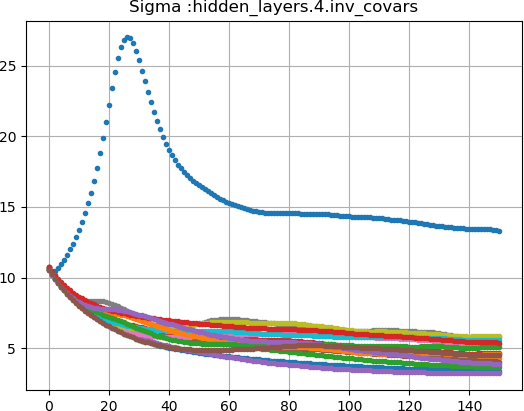
\includegraphics[width=\textwidth]{images/2D-network-toy/sigmas-change.png}
        \caption*{Changes to the FGNs' variances}
    \end{subfigure}
    \caption{Network parameters: 32-16 neurons in hidden layers, dropout layers with 1/16 drop rate, spherical variance $\sigma$ and 2-norm for the FGN. First FGN layer centers initialized to random data points.}
    \label{fig:toy-2d-params}
\end{figure}
 
\chapter{Experimental Results: FGNs over MNIST}
\label{Experimental Results: FGNs over MNIST}
With the behavior of FGNs verified on toy data, we now test it on real data, with the goal of providing defense against adversarial attacks. The first dataset tested is MNIST, a collection of handwritten digit images by LeCun et al. 2010 \cite{lecun-mnisthandwrittendigit-2010}. Three networks will be compared:
\begin{itemize}
    \item A network built with two fully-connected layers of 64 classical neurons each, with dropout layers with drop rate 0.2 in between each layer, and with a softmax output layer.
    \item A network built from FGNs directly converted from the classic network above, with no retraining, and with a variance $\sigma=10$ large enough to not modify the behavior over the training data.
    \item The same FGN network as above, retrained over the data for a single epoch with a tiny $\lambda=10^{-10}$ loss pressure to shrink the variances $\sigma$.
\end{itemize}
All three networks have over 99\% accuracy over the training data and over 97\% over the validation data. The specific network design choices (size and number of layers) are not relevant to the conclusions drawn, as other designs were tested with similar experimental results. The three networks were tested over two sets of randomized images: one built from images with fully randomized pixel values, which have different mean and variance compared MNIST; and the other built from images consisting of shuffled MNIST images, which preserve the mean and variance. Figure \ref{fig:randoms} shows image samples from these two sets.
\begin{figure}[!h]
    \centering
    \begin{subfigure}[t]{0.49\textwidth}
        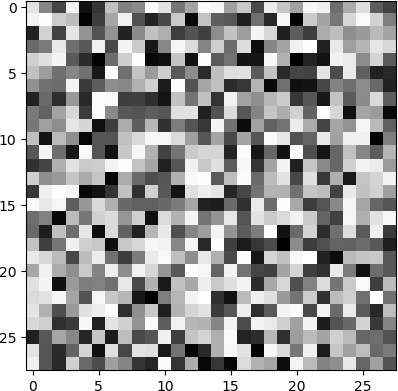
\includegraphics[width=\textwidth]{images/mnist-behavior/MNIST-Sample-random-noise-fixed.png}
        \caption*{Fully random pixels}
    \end{subfigure}
    \begin{subfigure}[t]{0.49\textwidth}
        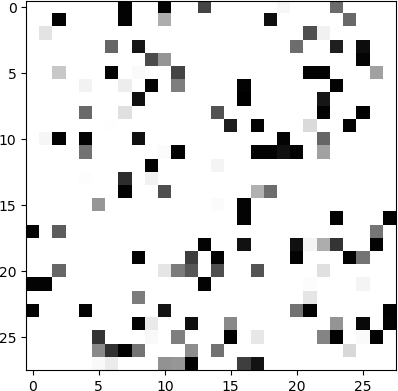
\includegraphics[width=\textwidth]{images/mnist-behavior/MNIST-Sample-random-shuffled-noise-fixed.png}
        \caption*{Shuffled MNIST image}
    \end{subfigure}
    \caption{Samples from the two randomized images datasets.}
    \label{fig:randoms}
\end{figure}

\section{Behavior over Random Images}
While the classical network has a high accuracy, it also has a high confidence in its predictions. Over the validation set, over 99\% of its predictions gave one of the ten digit classes a confidence greater that $0.5$ i.e. a majority confidence over all the other classes. In fact most of the predictions are well into the [$0.9,1.0$] confidence range, as shown by figure \ref{fig:classic-mnist}.
\begin{figure}[!h]
    \centering
    \begin{subfigure}[t]{0.49\textwidth}
        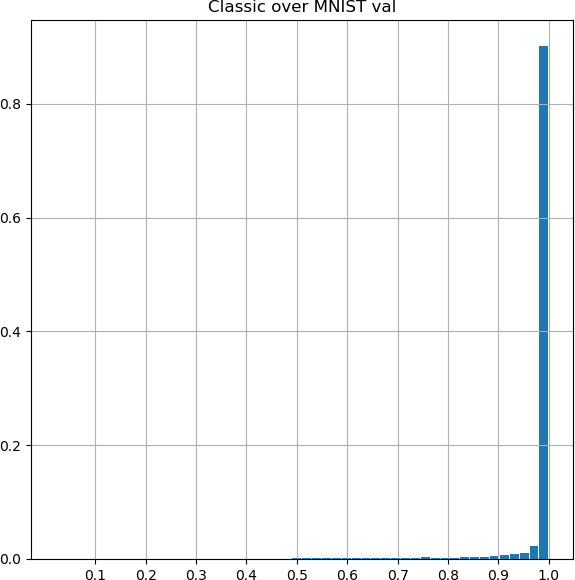
\includegraphics[width=\textwidth]{images/mnist-behavior/classic-hist-val.png}
        % \caption*{}
    \end{subfigure}
    \caption{Histogram of confidences - classic network.}
    \label{fig:classic-mnist}
\end{figure}\\
When the same network is tested over the randomized images sets, the histograms of confidences  \ref{fig:classic-hists} show that a majority of predictions still have above $0.5$ confidence, even though the randomized images are far away in the high dimensional hyper-space from the MNIST images. Figure \ref{fig:classic-preds} shows examples of randomized images, highlighting those given an MNIST digit class with over 0.9 confidence. This is replication of results from Szegedy et al. 2013 \cite{szegedy2013intriguing}.
\begin{figure}[!h]
    \centering
    \begin{subfigure}[t]{0.48\textwidth}
        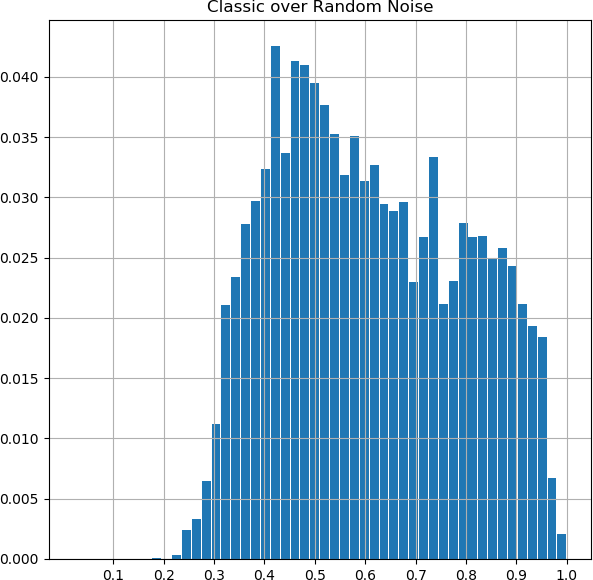
\includegraphics[width=\textwidth]{images/mnist-behavior/classic-hist-random.png}
        \caption*{Over 66\% of confidences $>0.5$}
    \end{subfigure}
    \begin{subfigure}[t]{0.48\textwidth}
        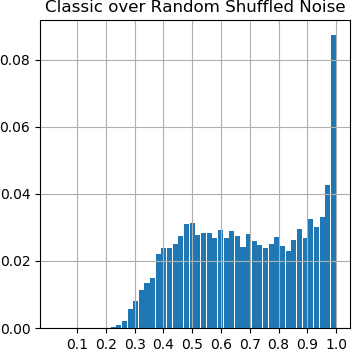
\includegraphics[width=\textwidth]{images/mnist-behavior/classic-hist-shuffled.png}
        \caption*{Over 78\% of confidences $>0.5$}
    \end{subfigure}
    \caption{}
    \label{fig:classic-hists}
\end{figure}
\begin{figure}[!h]
    \centering
    \begin{subfigure}[t]{0.48\textwidth}
        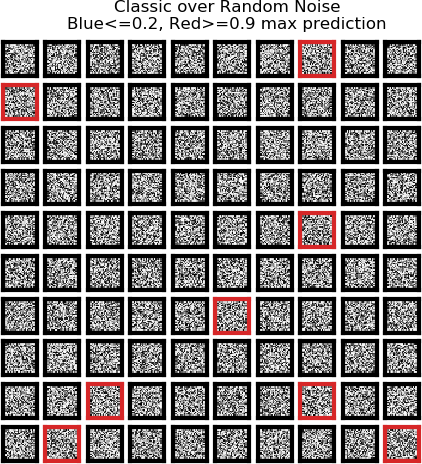
\includegraphics[width=\textwidth]{images/mnist-behavior/classic-pred-random.png}
        % \caption*{}
    \end{subfigure}
    \begin{subfigure}[t]{0.48\textwidth}
        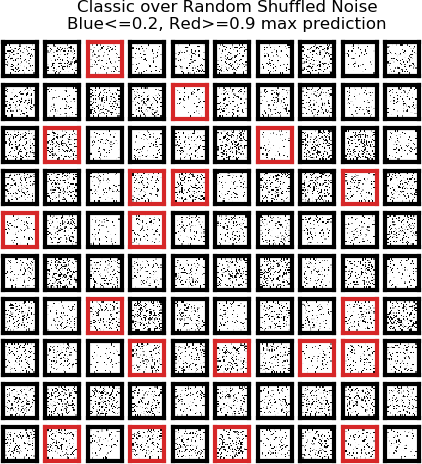
\includegraphics[width=\textwidth]{images/mnist-behavior/classic-pred-shuffled.png}
        % \caption*{}
    \end{subfigure}
    \caption{Sample over-confident predictions made by the classic network.}
    \label{fig:classic-preds}
\end{figure}
\newpage% explicit page break 

By design the converted FGN network does not modify the behavior of the classic network over the MNIST training data. It outputs identical values and the histogram of its prediction confidences over the validation data looks identical to that of classic network shown in figure \ref{fig:classic-mnist}. By contrast, when the converted FGN network is tested over the randomized images sets, the histograms are shifted towards lower values, with fewer confident predictions. These histograms are shown in figure \ref{fig:converted-hist}.
\begin{figure}[!h]
    \centering
    \begin{subfigure}[t]{0.49\textwidth}
        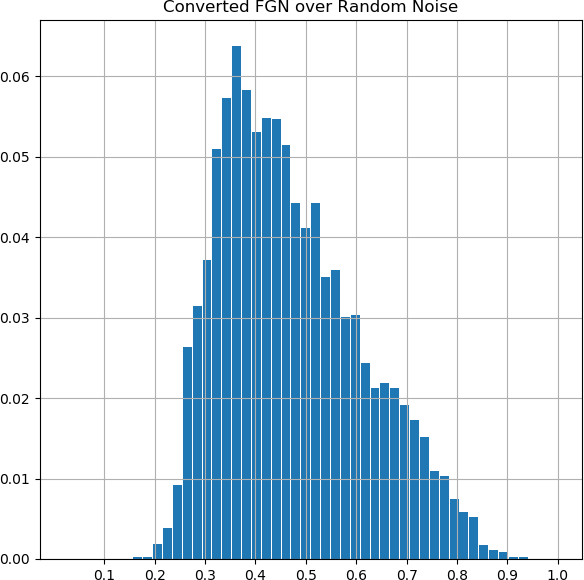
\includegraphics[width=\textwidth]{images/mnist-behavior/converted-hist-random.png}
        \caption*{Over 47\% of confidences $>0.5$}
    \end{subfigure}
    \begin{subfigure}[t]{0.49\textwidth}
        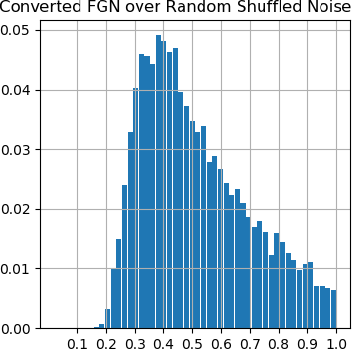
\includegraphics[width=\textwidth]{images/mnist-behavior/converted-hist-shuffled.png}
        \caption*{Over 45\% of confidences $>0.5$}
    \end{subfigure}
    \caption{}
    \label{fig:converted-hist}
\end{figure}

Finally, the FGN network is retrained over MNIST for a \emph{single} epoch. The pressure to shrink the variances $\sigma$ of the network's FNGs, added to the loss function, was a tiny $\lambda=10e^{-10}$. The overall accuracy remains the same (99\% over training data and 97\% over validation data) and still the network outputs extremely confident predictions over MNSIT images. The figure \ref{fig:retrained-mnist} is functionally identical to \ref{fig:classic-mnist}. But when this network is tested over the randomized image sets, almost all the predictions are at 0.1, as shown in figure \ref{fig:ret-hist}, meaning the retrained FGN network's softmax output is actually all zeros, and making no prediction for these randomized images that are far away in the high dimensional hyper-space from the MNIST images. The retrained FGN network is restricting its activity exclusively to zones of the hyper-space in which the training data is present. These zones are still large enough to generalize from the training data to the validation data.
\begin{figure}[!h]
    \centering
    \begin{subfigure}[t]{0.49\textwidth}
        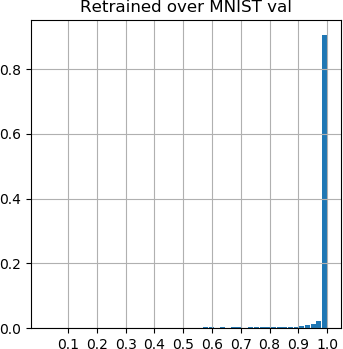
\includegraphics[width=\textwidth]{images/mnist-behavior/retrained-hist-val.png}
        % \caption*{}
    \end{subfigure}
    \caption{Histogram of confidences - retrained FGN network.}
    \label{fig:retrained-mnist}
\end{figure}
\begin{figure}[!h]
    \centering
    \begin{subfigure}[t]{0.49\textwidth}
        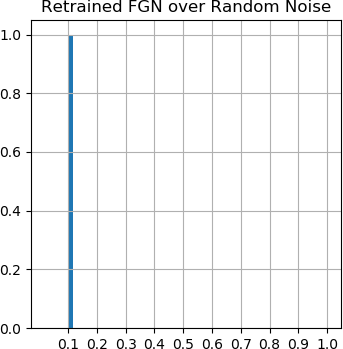
\includegraphics[width=\textwidth]{images/mnist-behavior/retrained-hist-random.png}
        \caption*{0.0\% of of confidences $>0.5$}
    \end{subfigure}
    \begin{subfigure}[t]{0.49\textwidth}
        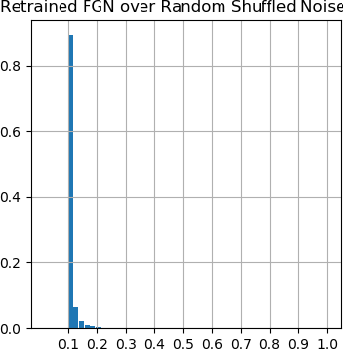
\includegraphics[width=\textwidth]{images/mnist-behavior/retrained-hist-shuffled-fixed.png}
        \caption*{0.05\% of confidences $>0.5$}
    \end{subfigure}
    \caption{}
    \label{fig:ret-hist}
\end{figure}
\newpage % explicit page break

Finally the three networks are tested on the EMNIST dataset, a collection of handwritten letter images by Cohen et al. 2017 \cite{cohen2017emnist}, a verification of the FGN behavior on out-of-domain samples. The histograms of the prediction confidences are shown in figure \ref{fig:hist-letters} and tell the same story as above: the classic models makes many confident predictions, the converted FGN network makes fewer, and the retrained FGN network makes none. Samples images are shown in figure \ref{fig:pred-letters}.
\begin{figure}[!h]
    \centering
    \begin{subfigure}[t]{0.32\textwidth}
        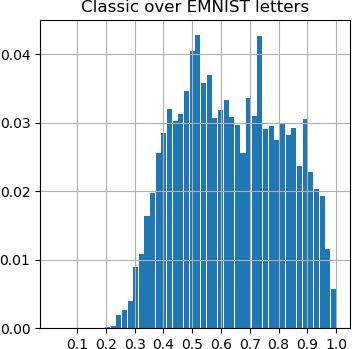
\includegraphics[width=\textwidth]{images/Letters/hist-classic-letters.png}
        \caption*{73\%  of confidences $>0.5$}
    \end{subfigure}
    \begin{subfigure}[t]{0.32\textwidth}
        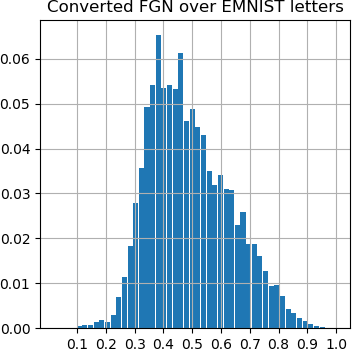
\includegraphics[width=\textwidth]{images/Letters/hist-converted-letters.png}
        \caption*{42\% of confidences $>0.5$}
    \end{subfigure}
    \begin{subfigure}[t]{0.32\textwidth}
        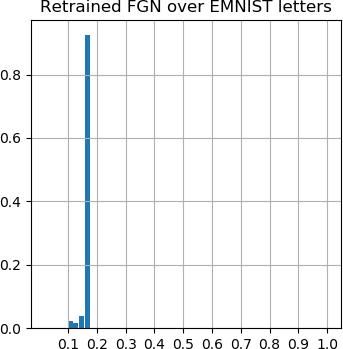
\includegraphics[width=\textwidth]{images/Letters/hist-retrained-letters.png}
        \caption*{0.0\% of confidences $>0.5$}
    \end{subfigure}
    \caption{}
    \label{fig:hist-letters}
\end{figure}
\begin{figure}[!t]
    \centering
    \makebox[\textwidth][c]{
        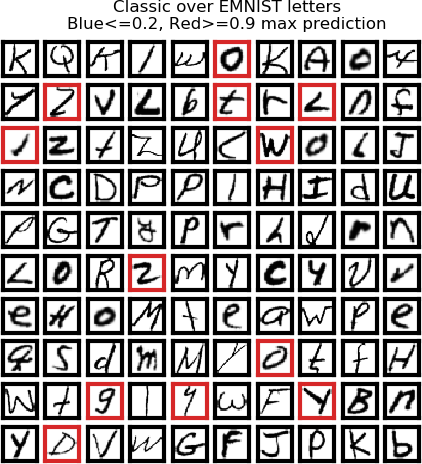
\includegraphics[width=0.40\textwidth]{images/Letters/classic-letters.png}
        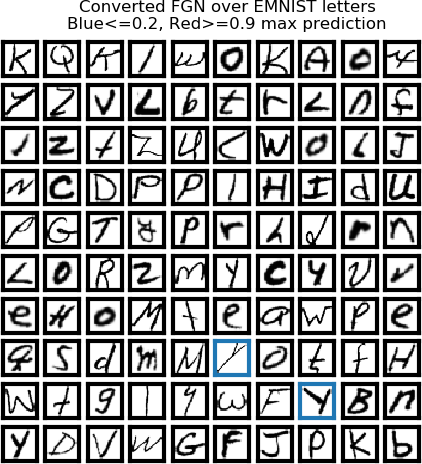
\includegraphics[width=0.40\textwidth]{images/Letters/converted-letters.png}
        \includegraphics[width=0.40\textwidth]{images/Letters/retrained-letters.png}
    }
    \caption{Sample EMNIST images with their prediction confidences given by the different networks. Note that some of the confident predictions by the classic network are on images of letters that resemble digits, yet it misses other. Humans would classify all the letter Os as the digit zero. By contrast the retrained FGN networks makes no confident predictions for any of the letters, regardless of how close they resemble digits to humans.}
    \label{fig:pred-letters}
\end{figure}
\newpage %explicit page break

\section{Protection against FGSM attack}
While protection from out-of-domain predictions is a useful feature of FGN networks, it does not guarantee protection from adversarial attacks. To verify this, the networks were tested against the untargeted FGSM attack first introduced by Goodfellow 2014 \cite{goodfellow2015explaining}, which generates adversarial examples by taking a single fixed-size step in the direction of the gradient of the loss with regards to the input image. An attack is considered successful if it both changes the class of the prediction outputted by the network for this input, and the confidence of the class is over 0.5. A parameter of the FGSM attack is $\epsilon$ the size of the fixed-length step, which also corresponds to the maximum amount of distortion allowed to the original image. Larger $\epsilon$ lead to a larger number of successful attacks but make the added adversarial noise more noticeable. The smallest step $\epsilon$ tested is equal to the smallest change possible to an 8-bit pixel. In addition to the three networks previously described in Chapter \ref{Experimental Results: FGNs over MNIST} (the classical network, the converted FGN network and the retrained FGN network), a fourth network is tested against FGSM. This network is built from the converted FGN network and is retrained for 100 epochs, the same number of epochs used to train the classical network, and with a much larger pressure $\lambda=10^{-5}$ to shrink the variances $\sigma$ of the FNGs added to the loss. This long-retrained FGN network maintains a 99\%/97\% accuracy during training/validation, with a high confidence in its predictions over MNIST.

The FGSM attack was run over the 10,000 images from the MNIST validation set. The results are shown in figure \ref{fig:fgsm-counts} and show that FGN networks are more resistant to the FGSM adversarial attack than the classic network. The long-retrained FGN network appears to be impervious the FGSM attack even for small $\epsilon$, while the classical network remains vulnerable to attacks not matter the $\epsilon$ value. For both the converted and the quick-retrained FGN networks, smaller $\epsilon$ values still allow for a comparable number of successful attacks as the classical network, but past a certain $\epsilon$ value are no longer vulnerable to the FGSM attack. Taking a closer look, all the outputs of the FGN networks on the adversarial images in the cases with no successful attacks are zeros, indicating that these adversarial images are falling outside of the range of the network FGNs. Figure \ref{fig:fgsm-compar} shows the evolution of the confidence in the adversarial predictions as $\epsilon$ increases.
\begin{figure}[!t]
    \centering
        \includegraphics[width=\textwidth]{images/successful-attacks-comparisons/succesful_fgsm_count.png}
    \caption{Count of successful FGSM attacks (changes the class, confidence$>0.5$) among the 10K MNIST validation set images.}
    \label{fig:fgsm-counts}
\end{figure}
\begin{figure}[!t]
    \centering
    \makebox[\textwidth][c]{
        \includegraphics[width=0.6\textwidth]{images/successful-attacks-comparisons/fgsm-comp-0.png}
        \includegraphics[width=0.6\textwidth]{images/successful-attacks-comparisons/fgsm-comp-2.png}
    }
    \makebox[\textwidth][c]{
        \includegraphics[width=0.6\textwidth]{images/successful-attacks-comparisons/fgsm-comp-3.png}
        \includegraphics[width=0.6\textwidth]{images/successful-attacks-comparisons/fgsm-comp-4.png}
    }
    \caption{Histograms of the confidences in the predictions over FGSM adversarial images for the classical network, the converted FGN network, and the long-retrained network. For $\epsilon=0$ the adversarial images are the same as the MNIST images and the networks output predictions with high confidence. For any non-zero $\epsilon$, the long-retrained FGN network outputs all zeros, while the classical network outputs high confidences. As $\epsilon$ increases, the converted FGN network starts behaving differently from the classical network, outputting lower confidences, until it matches the long-retrained FGN network and outputs all zeros. }
    \label{fig:fgsm-compar}
\end{figure}

\section{Observations}
\label{Observations}
While FGN networks offer some protection from FGSM attacks, it is unclear how the FGN networks are able to not overfit and generalize from training data to validation data, while making no predictions on adversarial images. To explore this phenomenon, figure \ref{fig:fgsm-bounds} plots two dimensional cross-sections of the 784 dimensional MNIST image space, filling the space with colors associated with digit classes as predicted by the networks. The images show movement along the FGSM attack vector starting from an MNIST image at the center, and a randomly chosen vector orthogonal to the attack vector. The half-width of the cross section was chosen to be $\epsilon=0.06$ as that is when the classical network and converted FGN network start behaving differently. 

For the classical network, boundaries between the original image predicted class and every other class are present, indicating the existence of many adversarial examples within the $\epsilon$-hypersphere around the image. The converted FGN network exhibits the same boundaries but with weaker confidence as we move away from the original image, making adversarial examples rarer. And the long-retrained FGN network makes no predictions anywhere except at the original image, making adversarial examples non-existent.
\begin{figure}[!t]
    \centering
    \makebox[\textwidth][c]{
            \includegraphics[width=0.43\textwidth]{images/observations/classic-bounds.png}
            \includegraphics[width=0.43\textwidth]{images/observations/converted-bounds.png}
            \includegraphics[width=0.43\textwidth]{images/observations/long-bounds.png}
    }
    \caption{Boundaries between predicted classes in the hyper-space for the classical network, the converted FGSM network and the long-retrained FGN network. Each small image is square 2D cross-section of the hyperspace, defined by an MNIST image at the center, the FGSM attack vector on the horizontal axis, and a random orthogonal vector on the vertical axis. The images are $2\epsilon$ wide. Each pixel is colored by the predicted class, with higher color intensity for higher confidence. This is example shows a digit 3 adversarially transformed into a digit 5 for the classical network and converted FGN network.\protect\footnotemark}
    \label{fig:fgsm-bounds}
\end{figure}

The lack of predictions around the MNIST image by the long-retrained FGN network seems to imply that the model is overfitting to the training data, but the high accuracy on the validation data already contradicts this. Figure \ref{fig:fgsm-img2img}, which plots cross-sections of the hyperspace while moving from one MNIST image to another, shows that both FGN networks make predictions continuously along the image-to-image vector, and rarely nearby, while the classical network makes confident predictions over the entire nearby space. It's notable that there are no areas of zero-valued predictions in between the images.\footnotetext{Larger version of images are available in the addendum.} 
\begin{figure}[!h]
    \centering
    \makebox[\textwidth][c]{
            \includegraphics[width=0.43\textwidth]{images/observations/classic-img8toimg4.png}
            \includegraphics[width=0.43\textwidth]{images/observations/converted-img8toimg4.png}
            \includegraphics[width=0.43\textwidth]{images/observations/long-img8toimg4.png}
    }
    \caption{Boundaries between predicted classes in the hyper-space for the classical network, the converted FGSM network and the long-retrained FGN network. Each small image is square 2D cross-section of the hyperspace, defined by a vector from one MNIST image at the leftmost center pixel to another MNIST image a the rightmost center pixel, and a random orthogonal vector on the vertical axis. Each pixel is colored by the predicted class, with higher color intensity for higher confidence. This is example shows a digit 8 linearly transformed into a digit 4.}
    \label{fig:fgsm-img2img}
\end{figure}

\chapter{Remaining Work}
These results indicated that FGNs provide neural network with resistance to adversarial attacks, but to further validate their usefulness, FGNs still need to be tested against attacks other than FGSM and on datasets other than MNIST.

The two most prevalent adversarial attacks besides FGSM are the Projected Gradient Descent (PGD) attack and the Carlini-Wagner attack. The PGD attack, described by Madry et al. 2015 \cite{madry2019deep}, is an iterated version of the FGSM attack. It is an expensive attack, but providing defense against it has potential to defende against all gradient-based attacks. The Carlini-Wagner attack by Carlini et al. 2017 \cite{carlini2017evaluating}, another gradient-based attack, is derived from testing various heuristics and tailored to commonly used distance metrics. 

To ensure that the current results against adversarial attacks are not dataset specific, FGN networks will be trained and attacked on the CIFAR-10 and SPEECHCOMMANDS datasets and associate tasks. The CIFAR-10 dataset by Krizhevsky et al. 2009 \cite{Krizhevsky2009LearningML} consists of color images larger than the MNIST images from ten classes such as TRUCK and CAT. The SPEECHCOMMANDS dataset by Pete Warden 2018 \cite{DBLP:journals/corr/abs-1804-03209} consists of audio files associated with shorts words such as YES and HOUSE. 

FGN networks should also provides defense transferring adversarial examples across networks, and against universal adversarial perturbations which are changes that can be applied to any input, as described by Moosavi-Dezfooli et al. 2017 \cite{moosavidezfooli2017universal}.

FGNs networks should also not rely on the specific fully-connected feedforward network architecture to provide defense against adversarial attacks. The convolutional layer, popularized by Krizhevsky et al. 2012 \cite{krizhevsky2012imagenet} with their Alexnet model, is an important component of modern neural networks and as such an FGN version of the convolutional layer will be implemented and tested.

Finally, continuing work on FGNs will shed more light on their properties, their best practices, and how they compare to other research. Of particular interest are understanding the FGN behavior in between data points and data classes, analyzing the best p-norm variants and ways to initialize the variances and centers, comparing to other rubbish class proof methods such as Bayesian neural networks (Mullachery et al. 2018 \cite{mullachery2018bayesian}), evaluating the FGN networks in term of calibration (Guo et al. 2017 \cite{guo2017calibration}),and finally comparing to recent adversarial defenses such fast-PGD by Wong et al. 2020 \cite{wong2020fast}.

%%% image template
% \begin{figure}[!htbp]
%     \centering
%     \makebox[\linewidth][c]{
%         \begin{subfigure}[t]{\textwidth}
%             \includegraphics[width=\textwidth]{}
%             \caption*{}
%         \end{subfigure}
%     }
%     \caption{Caption}
%     \label{fig:my_label}
% \end{figure}


%% If you want an introduction in the table of contents, but
%% without its own chapter number, do this:
%% \chapter*{Introduction}
%% \addcontentsline{toc}{chapter}{\numberline{}Introduction}
%% \markboth{Introduction}{INTRODUCTION}

%% Also, to ensure that the bibliography is in the table of
%% contents, do this when you reach the end of the main text:

\backmatter
%% \begin{thebibliography}{n} %(where n is the longest item)
%% \addcontentsline{toc}{chapter}{\numberline{}Bibliography }

\bibliographystyle{IEEEtran}
\bibliography{bibl.bib}

\chapter{Addendum}
\begin{figure}
    \centering
    \includegraphics[width=\textwidth]{images/observations/classic-bounds.png}
    \caption*{Larger version of images in figure \ref{fig:fgsm-bounds}.}
\end{figure}
\begin{figure}
    \centering
    \includegraphics[width=\textwidth]{images/observations/converted-bounds.png}
    \caption*{Larger version of images in figure \ref{fig:fgsm-bounds}.}
\end{figure}
\begin{figure}
    \centering
    \includegraphics[width=\textwidth]{images/observations/long-bounds.png}
    \caption*{Larger version of images in figure \ref{fig:fgsm-bounds}.}
\end{figure}
\begin{figure}
    \centering
    \includegraphics[width=\textwidth]{images/observations/classic-img8toimg4.png}
    \caption*{Larger version of images in figure \ref{fig:fgsm-img2img}.}
\end{figure}
\begin{figure}
    \centering
    \includegraphics[width=\textwidth]{images/observations/converted-img8toimg4.png}
    \caption*{Larger version of images in figure \ref{fig:fgsm-img2img}.}
\end{figure}
\begin{figure}
    \centering
    \includegraphics[width=\textwidth]{images/observations/long-img8toimg4.png}
    \caption*{Larger version of images in figure \ref{fig:fgsm-img2img}.}
\end{figure}


\end{document}